% A Sample Thesis for the University of Calgary
% =============================================

% This is a sample LaTeX document to build a University of Calgary
% graduate thesis according to the guidelines of the Faculty of
% Graduate Studies, available here:
% https://grad.ucalgary.ca/current-students/thesis-based-students/thesis/building-thesis

% To use this sample for your own thesis, rename this file, make any changes
% necessary, then add the content of your thesis t othe included files
% frontmatter.tex, chapter1.tex, etc.

% First, we load the UCalgary Memoir Thesis class ucalgmthesis,
% available at https://github.com/rzach/ucalgmthesis

% By default (without options), this produces a 1-1/2 spaced thesis in
% 11 point font without running heads. See the README file for a
% description of all package options.

% In our sample we give three options: Option utopia sets the thesis in a
% nice font. Option headers produces running heads. Option manuscript
% formats the page in a way suitable for reading and commenting: 12 pt type,
% double spaced, approx. 25 lines per page, with approx. 72 characters
% per line. For filing in the Vault, remove that option to produce a
% more compact thesis with a slightly better layout.

\documentclass[utopia,headers,manuscript]{ucalgmthesis}

% Using LaTeX? Then you're probably using math, and so you want to use
% the AMS math commands and define some theorem environments! But you
% can take these out or use your own favorite theorem package.

\usepackage{amsmath,amsthm}

\newtheorem{thm}{Theorem}
\theoremstyle{definition}
\newtheorem{defn}[thm]{Definition} % please number all of them together!

% microtype makes everything look better

\usepackage{microtype}

% We'll need some colored links, so we load xcolor and hyperref. But
% you can take that out if you don't want links at all.

\usepackage[dvipsnames]{xcolor}

% You can turn off the boxes around links made by hyperref. Then links
% will appear in a different color, and per guidelines, all links must
% be blue or black. For blue links say

\usepackage[colorlinks,allcolors=MidnightBlue]{hyperref} 

% For black links, 
% \usepackage[hidelinks]{hyperref}

% If you prefer hyperref's boxes around links (which don't print), you
% can also change their color. With boxes around links, you probably
% don't want everything in the table of contents to be a link, so we
% only make the page numbers links.
%
% \usepackage[allbordercolors=Periwinkle,linktocpage]{hyperref}

% The table of contents in your PDF reader's sidebar is just titles by
% default, but it's nice to also have chapter and section numbers for
% easy navigation.

\usepackage[numbered]{bookmark}

% For author-year references, you probably want to use natbib with a
% bibliography style appropriate for your discipline; or check out
% latexbib!

\usepackage[round]{natbib}


% more packages

\usepackage{tikz-cd}
\usepackage{cancel}
\usepackage{csquotes}


\let\lif\to
\def\peirceor{\mathbin{\ooalign{$\smile$\cr\hfil$\mid$\hfil}}}

% Now we put in the information for the thesis title page.

% Full Name

\author{Brent C. Odland}

% Full Title

\title{Peirce's Triadic Logic: Continuity, Modality, and L}

% Official name of the degree

\degree{MASTER OF ARTS}

% The name of the graduate program (not the department!)

\prog{Graduate Program in Philosophy}

% The month (for the final version: when you file, not when you defended)

\monthname{JUNE}

% The year

\thesisyear{2020}

% Tell hyperref to put author and title into the PDF metadata

\hypersetup{pdfinfo={Title={\thetitle},Author={\theauthor}}}

% Often you only want to output a single chapter so you can send it to
% your supervisor. Use includeonly and make sure everything you don't
% always want compiled to PDF is include'd from a separate file. For
% instance, to produce a PDF only of chapter 1, endnotes and
% bibliography, say

%\includeonly{ch-introduction,backmatter}
%\includeonly{ch-description-of-notes,backmatter}
%\includeonly{ch-philo-motivation,backmatter}
%\includeonly{ch-continuity,backmatter}

% To compile only the title page, which you need when submitting your
% thesis, say

% \includeonly{titlepage}

% and then copy the resulting PDF to a separate file.

\begin{document}

\frontmatter

% titlepage.tex just makes the titlepage; it's in its own file so you
% can typeset it alone using includeonly.

% Sample University of Calgary Thesis
% This file contains the TITLE PAGE

\makethesistitle


% frontmatter.tex contains the abstract, preface, acknowledgments, and
% the commands to produce the table of contents, list of tables, etc.

%% Sample University of Calgary Thesis
% This file contains the FRONT MATTER other thna the title page

\chapter{Abstract}

In 1909, in his \textit{Logic Notebook}, Charles Sanders Peirce conducted what, to my knowledge, are the first experiments with many-valued post-Aristotelian logic. As these experiments are entirely contained in a handful of pages in his notebook, which were not published or discussed by other authors during his lifetime, his reasons are open to conjecture. By examining and transcribing these pages and connecting them to his larger body of philosophy, I show how his motivations lie within his views on modality, continuity, and his hypothetical cosmology.


\chapter{Preface}

All of the images contained in this thesis come from the \textit{Charles S. Peirce Papers} collection in the Houghton Library at Harvard. These images have been made freely available as part of the Houghton Library's \textit{Digitization Initiative}. Most of the primary sources for this project come from \textit{The Collected Papers of Charles Sanders Peirce. Electronic Edition}. Much of the information used in this thesis comes from the articles ``Peirce's Triadic Logic", by Max Fisch and Atwell Turquette \citeyearpar{fisch_peirces_1966}, and ``Peirce's Triadic Logic Re-visited", by Robert Lane \citeyearpar{lane_peirces_1999}. The diagram in Chapter 2, Section 2, is a modified version of a diagram presented by Turquette in \citeyear{turquette_dualism_1972}.

This thesis is original, unpublished, independent work by the author,
Brent C. Odland.
  
\chapter{Acknowledgments}


I would like to thank my supervisor, Mark Migotti, for guiding me through the whole process of writing this thesis and patiently listening to the crazy ideas I brought to him before settling on this topic. I would also like to thank Richard Zach, who went far above and beyond the ``duties" of an unofficial co-supervisor throughout the course of this project. Thank you to Nicole Wyatt for reading this thesis and offering helpful suggestions toward its improvement. Thank you also to Jen Smith, for facilitating all of the administrative work that goes into a project like this. Thank you to Anne Levey, for all your support and advice throughout the entirety of my MA. And thanks to my wife, Emma Ritchie, for her constant support and encouragement.

\dedication{For the poor tortoise, who had to wait while Achilles took all his teeny tiny little steps.}

\tableofcontents

\chapter{List of Abbreviations}

\begin{center}
\begin{tabular}{ c c } 

 AFC & \textit{A Fourth Curiosity} \\ 
 CCL & \textit{Cambridge Conference Lectures} \\ 
 CP & \textit{Collected Papers of Charles Sanders Peirce} \\
 EP & \textit{Essential Peirce} \\ 
 L & Refers to letter numbers from \textit{The Robin Catalogue}\\ 
 MS & Refers to manuscript numbers from \textit{The Robin Catalogue}\\ 
 NEM & \textit{New Elements of Mathematics} \cite{peirce1976new} \\ 
 PEM & Principle of excluded middle \\ 
 PC & Principle of non-contradiction \\ 
\end{tabular}
\end{center}

% If you have no tables, delete the next line

%\listoftables

% If you have no figures, delete the next line

%\listoffigures

% Consult Ch 9 of the memoir class manual on how to set up other
% content lists. Note that memoir does not automatically clear the
% page for these. ucalgmthesis fixes this for the default table of
% contents and lists of tables and figures, but not for anything you
% define


% The main matter of the thesis contains the actual content, separated
% into chapters.

\mainmatter

\chapter{Introduction \\ \small{Charles Sanders Peirce: Logician, Philosopher, and Beyond}}
Charles Sanders Peirce is probably best known as founder of the increasingly popular school of thought in philosophy  called pragmatism. He was far more obscure in his day and likely would have been completely so if it were not for his close friend, William James, who adapted and popularized some of Peirce's ideas (most notably his Pragmatic Maxim). In fact, Peirce's claim to fatherhood might be contested, as it was James who first brought pragmatism to general audiences.\footnote{Peirce ended up disliking James' version of the doctrine so much that in 1905, he began to call his own version ``pragmaticism," to distance himself from James and other pragmatists (CP 5.414).} While Peirce and James were dear friends, they differed sharply on some issues, especially on the nature of truth as prescribed by their pragmatism. Another area where the two differed was on metaphysics, where James was a nominalist and Peirce an adamant scholastic realist. Peirce was initially skeptical of metaphysics, but as time went on he devoted increasingly more thought to it. By the end of his life he had constructed a grand theory of speculative cosmology, incorporating a rich triadic ontology.

As a philosopher, Peirce was insightful, ambitious, and exceptionally creative. However, his complexity and penchant for inventing new technical terms sometimes led to an underwhelming reception of his work. The fact that the number of published works are dwarfed by the wealth of manuscripts, speculating on all manner of things from religion to logic machines, makes matters difficult for the Peirce scholar. The difficulty of Peirce scholarship is nicely summed up by this anecdote from a book review on a volume produced by Edward Moore and Richard Robin:\begin{quote} \noindent``There is a story that when Peirce retired to Milford, he built an attic study in his house accessible only by ladder. When the creditors that plagued his later years came calling, Peirce retreated to uninterrupted philosophizing by climbing to his study and drawing up the ladder behind him.

This story suggests a moral: the student of Peirce is often in a position like that of the bill collector. Access to Peirce can be difficult'' \citep[73]{thayer_book_1967}.\end{quote}

As this story betrays, Peirce led a troubled life. It is ironic that now we know him primarily as a philosopher, as in his own lifetime he made his living primarily as a working scientist.\footnote{A further irony can be found in the fact that a working scientist would embrace such a flamboyantly speculative metaphysics.} The only academic position he held was his appointment as a lecturer at Johns Hopkins. He held this position from 1879 until 1884, when he was fired for reasons tied to his divorce and subsequent marriage of his second wife Juliette \citep{hoopes_review_1999}. His isolation from the academic community partially explains the difficulty of his philosophy. There were few with whom he could test out ideas with. His student and long time correspondent and co-author, Christine Ladd-Franklin once wrote: \begin{quotation}\noindent``If Charles S. Peirce had happened to have a longer period of activity at the Johns Hopkins University---if the years had not been cut off during which he was kept upon the solid ground of intelligible reason by discussions with a constantly growing group of level-minded students,---there is no doubt that his work would have been of more certain value than it can be affirmed to be now'' \citep{ladd-franklin_charles_1916}.\end{quotation} Despite his tenuous academic career, Peirce remained keenly interested in philosophy, devoting all of his time to it when he was not working on the intellectual odd jobs he used to sustain himself.

The subject which he was hired to lecture on and which he taught Ladd-Frankin, O.H. Mitchell, John Dewey, and others, was logic. Peirce has been somewhat pushed out of the history of logic by the towering presence of Frege and Russell. His importance in the history of logic was, for a long time, not well understood until the  pioneering work on the subject by \citet{Dipert1995-DIPPUP} and \citet{hintikka_place_1997}  was published. As a logician, Peirce worked within the algebraic tradition, which finds its roots in Boole's algebra of logic. He and Mitchell, discovered quantification independently of Frege. It is unclear when Peirce made this discovery, but it was no later than 1883 \citep{mitchell_new_1883}.\footnote{Interestingly, at the time quantification was apparently more obvious an advancement than we typically understand now. Frege never especially touted this achievement, nor does he use the phrase `quantification' to describe any aspect of his logic \citep{Dipert1995-DIPPUP}. Peirce seems to be the first person to specifically discuss quantification \citep{putnam_peirce_1982}.} He showed that propositional logic is expressively complete under a single operator, which we now refer to as ``Peirce's Arrow.'' Furthermore, the notation he and his pupils used was appreciated and expounded by Schröder and is only a typographical variant of the notation logicians currently use \citep{putnam_peirce_1982}. Löwenheim proved his famous theorem in this notation; and Zermelo wrote his axiomatic set theory in it (Ibid).

Peirce also appears to be the first person to distinguish between first and second order logics (Ibid); and even attempted to work with non-classical logics to deal with issues like modality. This brings us to the topic of my thesis.

In 1909, from around January 7th to February 23, Peirce began experimenting with three-valued logic, anticipating the pioneering work on the subject by  Łukasiewicz (\citeyear{Lukasiewicz1920}, translated in \citeyear{Lukasiewicz1970a}) and Post (\citeyear{post_introduction_1921}) by about 10 years. Łukasiewicz and Post arrived at their three-valued logic by generalizing the matrix method for defining truth functions to three values, a method that Peirce himself originated \citep{anellis_peirces_2012}. Now, Peirce's work on three-valued logic is nowhere near as sustained and complete Łukasiewicz's or Post's. It only spans 6 handwritten pages in Peirce's logic notebook. Nonetheless, when we observe Peirce wrestling with how to handle an additional truth value, this is striking and speaks to what we might call his logical instincts. It seems a natural question to ask why he saw fit to do this. What concerns had Peirce hoped to address with his three-valued logic (which he terms `triadic logic')? This is the question I hope to address throughout the course of this thesis.

The reasons others have taken up three-valued logics are quite diverse. Some, Łukasiewicz most notably, have been motivated by worries about future contingent propositions.  Some use an additional truth value in an attempt to deal with vague predicates and the Sorites Paradox. Others thought that results in quantum mechanics necessitated a third value. And others still have wanted to accommodate undecideable statements in mathematics. Generally speaking, in mainstream treatment of three-valued logic, the third value is meant to account for either possibility, accounting propositions that could turn out either to be true or false, or a kind of borderline indeterminacy, where propositions are really neither true or false. The fact that Peirce writes so little about what he was trying to capture makes the question of his motivations an interesting one.

The strongest indication of what is motivating Peirce to conduct his three-valued experiments comes from the last of the connected pages in his notebook. There he gives two indications that at a glance appear to take us in entirely distinct directions. The chief aim of this thesis is to rebut this view and demonstrate that there is an intimate connection between these two lines of thought.

The first indication is this statement characterizing his triadic logic: ``Triadic Logic is that logic which, though not rejecting entirely the Principle of Excluded Middle, nevertheless recognizes that every proposition, $S$ is $P$, is either true or false, \textit{or else S has a lower mode of being such that it can neither be determinately $P$, nor determinately not $P$, but is at the limit between $P$ and not $P$}'' (MS 339)\footnote{Throught this document I will often refer to passages written by Peirce in published and unpublished collections. It will be convenient to use the typical abbreviated citations for these. Passages from \textit{The Collected Papers of Charles S. Peirce} will be referred to in the text by CP v.p, where v is the volume and p is the paragraph number. Citations from \textit{New Elements of Mathematics} will be abbreviated to NEM v:p, where p will be the page number. \textit{The Essential Peirce} by EP x:y where x is the volume and y is the entry number. Unpublished manuscripts will be referred to as MS followed by the manuscript number. Most references to unpublished manuscripts will be to MS 339, Peirce's logic notebook. I refer to these pages by seq.xyz, according to the order in which they appear in the Harvard Mirador reproduction of this manuscript.} (My emphasis). Peirce's modes of being are another symptom of what has been called his triadism: his insistence in making tripartite divisions in virtually every aspect of philosophy. In his view there are precisely three modes of being, and these have a strictly modal interpretation. The first is possibility, second is actuality, and third is roughly necessity. He believed these modes of being applied to ideas as well as things in nature. Because these subjects have a lower mode of being, they are at the limit between the predicate and its denial. These propositions receive the third truth value, $L$, which is to be interpreted as limit, or not \textit{determinately} true nor false.
%Think about ditching explanation of modes of being. Maybe just use future contingents 
%Peirce's modes of being are another symptom of what has been called his triadism: his insistence in making tripartite divisions in virtually every aspect of philosophy. In his view their are precisely three modes of being, and these have a strictly modal interpretation. The first is possibility, second is actuality, and third is roughly necessity. He believed these modes of being applied to ideas as well as things in nature.

The second indication comes from a rather odd example on the same page: ``Thus, a blot is made on a sheet. Then every point of the sheet is unblackened or blackened. But there are points on the boundary line; and these points are incapable of being unblackened or of being blackened, since these predicates refer to the area about $S$ and a line has no area about any point of it'' (MS 339). Reserving discussion of the oddities of this example for later, it will become clear in subsequent chapters that it is connected to Peirce's views on continuity, continua, and breaches of continuity.

Peirce's understanding of continuity is a somewhat vexed topic. Throughout his life, and especially in the last 25 years, he constantly revised and re-evaluated his definition of it. In the mathematical sense, he came to understand continuity in about the same way as Cantor or Dedekind. However, Peirce's interest in continuity went far beyond mathematics. It extended to time, modality, and plays a central role in his hypothetical cosmology. All of this stems from a doctrine he endorsed and called synechism, which he held some version of going back as far as 1868 (CP 6.103, see also EP 1:2-4). Synechism, in Peirce's words, is ``the tendency to regard everything as continuous'' (EP 2:1). We will briefly see the genesis of his definition of continuity in Chapter 3, Section 2, and see how time, modality and cosmology fit into it in Chapter 4.

So far there have been two attempts to explain Peirce's philosophical motivations behind triadic logic; the first is due to Max Fisch and Atwell Turquette \citeyearpar{fisch_peirces_1966}, the second is due to Robert Lane \citeyearpar{lane_peirces_1999}. Each of these accounts takes a different one of the just mentioned clues as a starting point and arrive at seemingly distinct conclusions. Fisch and Turquette link Peirce's comment about modes of being to his special theory of modality, called `triadic modality.' Lane, on the other hand, denies that triadic modality figures into Peirce's motivations, and instead tries to locate the project entirely within his views on continuity.

Fisch, Turquette, and Lane have focused only on the three pages in Peirce's logic notebook in which he explicitly uses a third truth value. However, there are additional pages that are clearly connected to his triadic logic that can be included in this discussion. Since a digital version of the notebook has now been published \href{https://iiif.lib.harvard.edu/manifests/view/drs:15255301$637i}{online}, it is now much easier to examine these pages and present evidence that better allows us to determine Peirce's motivations. In light of this evidence, I will argue that the two seemingly opposed views on this topic are not actually incompatible and present a synthesis that brings us much closer to Peirce's true motivations.

%Be briefer and don't go into specific 

In the next two chapters I will survey and critically review nearly\footnote{Some of Turquette's papers have been cited but not discussed. Many of these papers are dedicated to purely formal results that can be generated from the page I refer to as seq.640. While these results are not uninteresting, it is highly unlikely that Peirce would have been aware of them and so are unlikely to help advance our understanding of what triadic logic was intended for in the first place. However, I have included discussion of Turquette's findings which Peirce might feasibly have noticed or known about.} all of  what has so far been written about Peirce's triadic logic. I will begin with what Peirce himself wrote in connection with this logic and then turn to more recent work on the topic by Turquette, Fisch, and Lane.

In Chapter 2 I give as close to an exhaustive presentation of Peirce's experiments in his notebook as possible. The first three pages I discuss have been taken up by the commentators just mentioned. The first of these is usually thought to mostly be a failed experiment, although it did yield some useful one-place operators. The second more successfully defines a set of three-valued connectives, all versions of conjunctions and disjunctions. The final page contains Peirce's most explicit statement of what his triadic logic was intended for and seems to reference some of his comments on both triadic modality, as well as continuity. Out of these three pages, the first two are \textit{versos} and only the third is a \textit{recto}.

%In the second half of chapter two, I discuss pages that are connected with triadic logic, but that the above commentators have left out of there discussion. The first of these contains examples of Peirce's existential graphs, his preferred representation of logic, but with an additional operator that does not appear to be used elsewhere. Peirce seems pretty quickly to have decided his graphical representation was not up to the job, as he reverted back to his symbolic notation on all subsequent pages. The second of these unmentioned pages makes reference to ``special universes'' as well as the ``fundamental quadratic'' of Boolean logic. The third of these seems to be mostly scratchwork with a concluding remark about functions on values being ``known'' and ``generally known.'' All three of these pages are \textit{rectos}, the first two of which are on the front side of the \textit{versos} in the first half of the section.

In chapter 3, I discuss Fisch and Turquette's paper, ``Peirce's Triadic Logic,'' and Lane's response, ``Peirce's Triadic Logic Revisited.'' These are the most well known accounts that attempt to describe the philosophical issues that may have motivated Peirce to experiment with three-valued logic. Fisch and Turquette are right that the notebook pages make a compelling case that triadic logic is connected with notions of modality and Peirce's tychism. After reviewing this, I turn to Lane's alternative account of Peirce's motivations. While I agree with Lane that continuity is an important piece of the puzzle, I argue against his claim that modality has nothing to do with it. Removing modality from our consideration entirely would involve ignoring an important part of the little historical evidence we have for why Peirce invented triadic logic. I conclude the section by providing evidence that demonstrates that the claim that Peirce was motivated by modality and the claim that he was motivated by continuity are in fact compatible. This view meshes well with much of Peirce's  other discussion of continuity and continua.

In the final chapter, I work out this view and show that we cannot properly understand the purpose of Peirce's triadic logic exclusively through modality or continuity alone. In the first section, I explain why Peirce thought his subject matter required him to deviate from classical logic. In the second, I answer the question as to why he needed his additional truth value, $L$. In the third, I give examples of the kinds of propositions that would be evaluated as $L$. I admit that this unification is by no means seamless. However, this is not necessarily a deficiency for this account but rather a natural result of its subject matter. Peirce's triadic logic was based on ideas that he himself never fully worked out to his own satisfaction. He continued writing about the ideas expressed here until he died in 1914 and he was proud to admit his own uncertainty.

%\chapter{Peirce's Notes on Triadic Logic}

%It is no secret that Peirce never reached the level of success that would have allowed him to publish as voluminously as he wrote within his lifetime.

%As such, 
Peirce's mature philosophy, along with his work on logic and set theory, is contained within a collection of unpublished manuscripts. One of these manuscripts, simply entitled ``The Logic Notebook,'' was a notebook where Peirce first set out and tested his ideas. Peirce wrote in this notebook periodically for most of his life. The first entry is dated November 12, 1865, while the final entry does not occur until November 1, 1909. At some point, these notes were separated and scattered amongst several files and remained  that way until the notebook was reassembled by Don Roberts in \href{https://iiif.lib.harvard.edu/manifests/view/drs:15255301$1i}{1961}. By 1964 they were reproduced on microfilm for viewing. Now images of the pages have been reproduced \href{https://iiif.lib.harvard.edu/manifests/view/drs:15255301$637i}{online}\footnote{https://iiif.lib.harvard.edu/manifests/view/drs:15255301$637i} as part of the Houghton Library's digitization initiative at Harvard. It is in this notebook that we find the three pages that have garnered Peirce attention for being an early pioneer of many-valued logic.

The first two pages where the use of a third truth value appear are both undated \textit{versos}. They were likely written between January 7th, 1909, and February 17th, 1909, judging by the dates on the other surrounding pages. The \textit{recto} between the two \textit{versos} is dated February 16th, and the one following the second page is dated the 17th. Of the pages Fisch and Turquette draw attention to, the only one that has been dated is  February 23rd, 1909. Fisch and Turquette were the first to notice and publish these pages in \citeyear{fisch_peirces_1966}.

All of the research on Peirce's triadic logic so far has focused on these three pages, however further examination of the surrounding pages reveals some obvious connections between triadic logic and other topics Peirce was working out at the time. The reason that most scholarship has neglected the other relevant pages is unclear. It is likely due to the fact that those were the only pages Fisch and Turquette decided to focus on when they wrote the first paper on the subject \citep{fisch_peirces_1966}. Since access to the original manuscript pages was limited until recently, their decision is likely the reason other scholars do not seem to have noticed these other pages. As ``The Logic Notebook'' had already been reassembled by the time Fisch and Turquette were writing, it is unlikely that they would not have seen the additional pages, which makes their decision not to mention them puzzling. 

The present chapter is devoted to providing an accurate description of the relevant pages from ``The Logic Notebook.'' I will first take up the three pages that have received the most discussion from other researchers on the subject. I will then discuss the additional pages that have hitherto been omitted. Throughout the section I will sometimes use numbers in parenthesis to indicate the parts on the page under current discussion. These numbers correspond to the numbers on the annotated images of the pages given as figures in their respective sections. The order in which the pages are discussed is not exactly the order they were chronologically written. I give priority to the pages that have already been taken up by others before examining those that have not. The order they likely would have been arranged when the notebook was in its original condition can be determined by reference to their seq. numbers. The first page related to Peirce's triadic logic is \href{https://iiif.lib.harvard.edu/manifests/view/drs:15255301$637i}{seq. 637} and the last is \href{https://iiif.lib.harvard.edu/manifests/view/drs:15255301$645i}{seq. 645}. It is possible that the undated \textit{versos} could have been afterthoughts, written after Peirce had come back and reflected upon the dated pages. There is one page that falls within the range between seq. 637--645 that I have not included in this discussion. That is \href{https://iiif.lib.harvard.edu/manifests/view/drs:15255301$643i}{seq. 643}, which is entitled ``Geometrical Topics."\footnote{This page was excluded because it did not initially appear to be relevant to Peirce's triadic logic. However, as Peirce's intentions become clearer, in light of this thesis, it might turn out to be relevant after all.} In the pages leading up to the triadic logic notes, Peirce was making notes on a paper for the American Mathematical Society, that was to be called ``Logical Remarks on Some Mathematical Definitions" (\href{https://iiif.lib.harvard.edu/manifests/view/drs:15255301$631i}{seq. 631} and onward). This paper does not appear ever to have been completed or published. The page immediately following the triadic logic notes, is a ``Note on the Tinctures," which turns out to be related to another system of logic, Peirce's Tinctured Gamma Graphs (\href{https://iiif.lib.harvard.edu/manifests/view/drs:15255301$646i}{seq. 646}).\footnote{See \cite{pietarinen_peirces_2006} for discussion of Tinctured Graphs.}
%Squeeze this down, the surrounding pages give great evidence...

\section{seq. 638 V.}

\begin{figure}
    \centering
    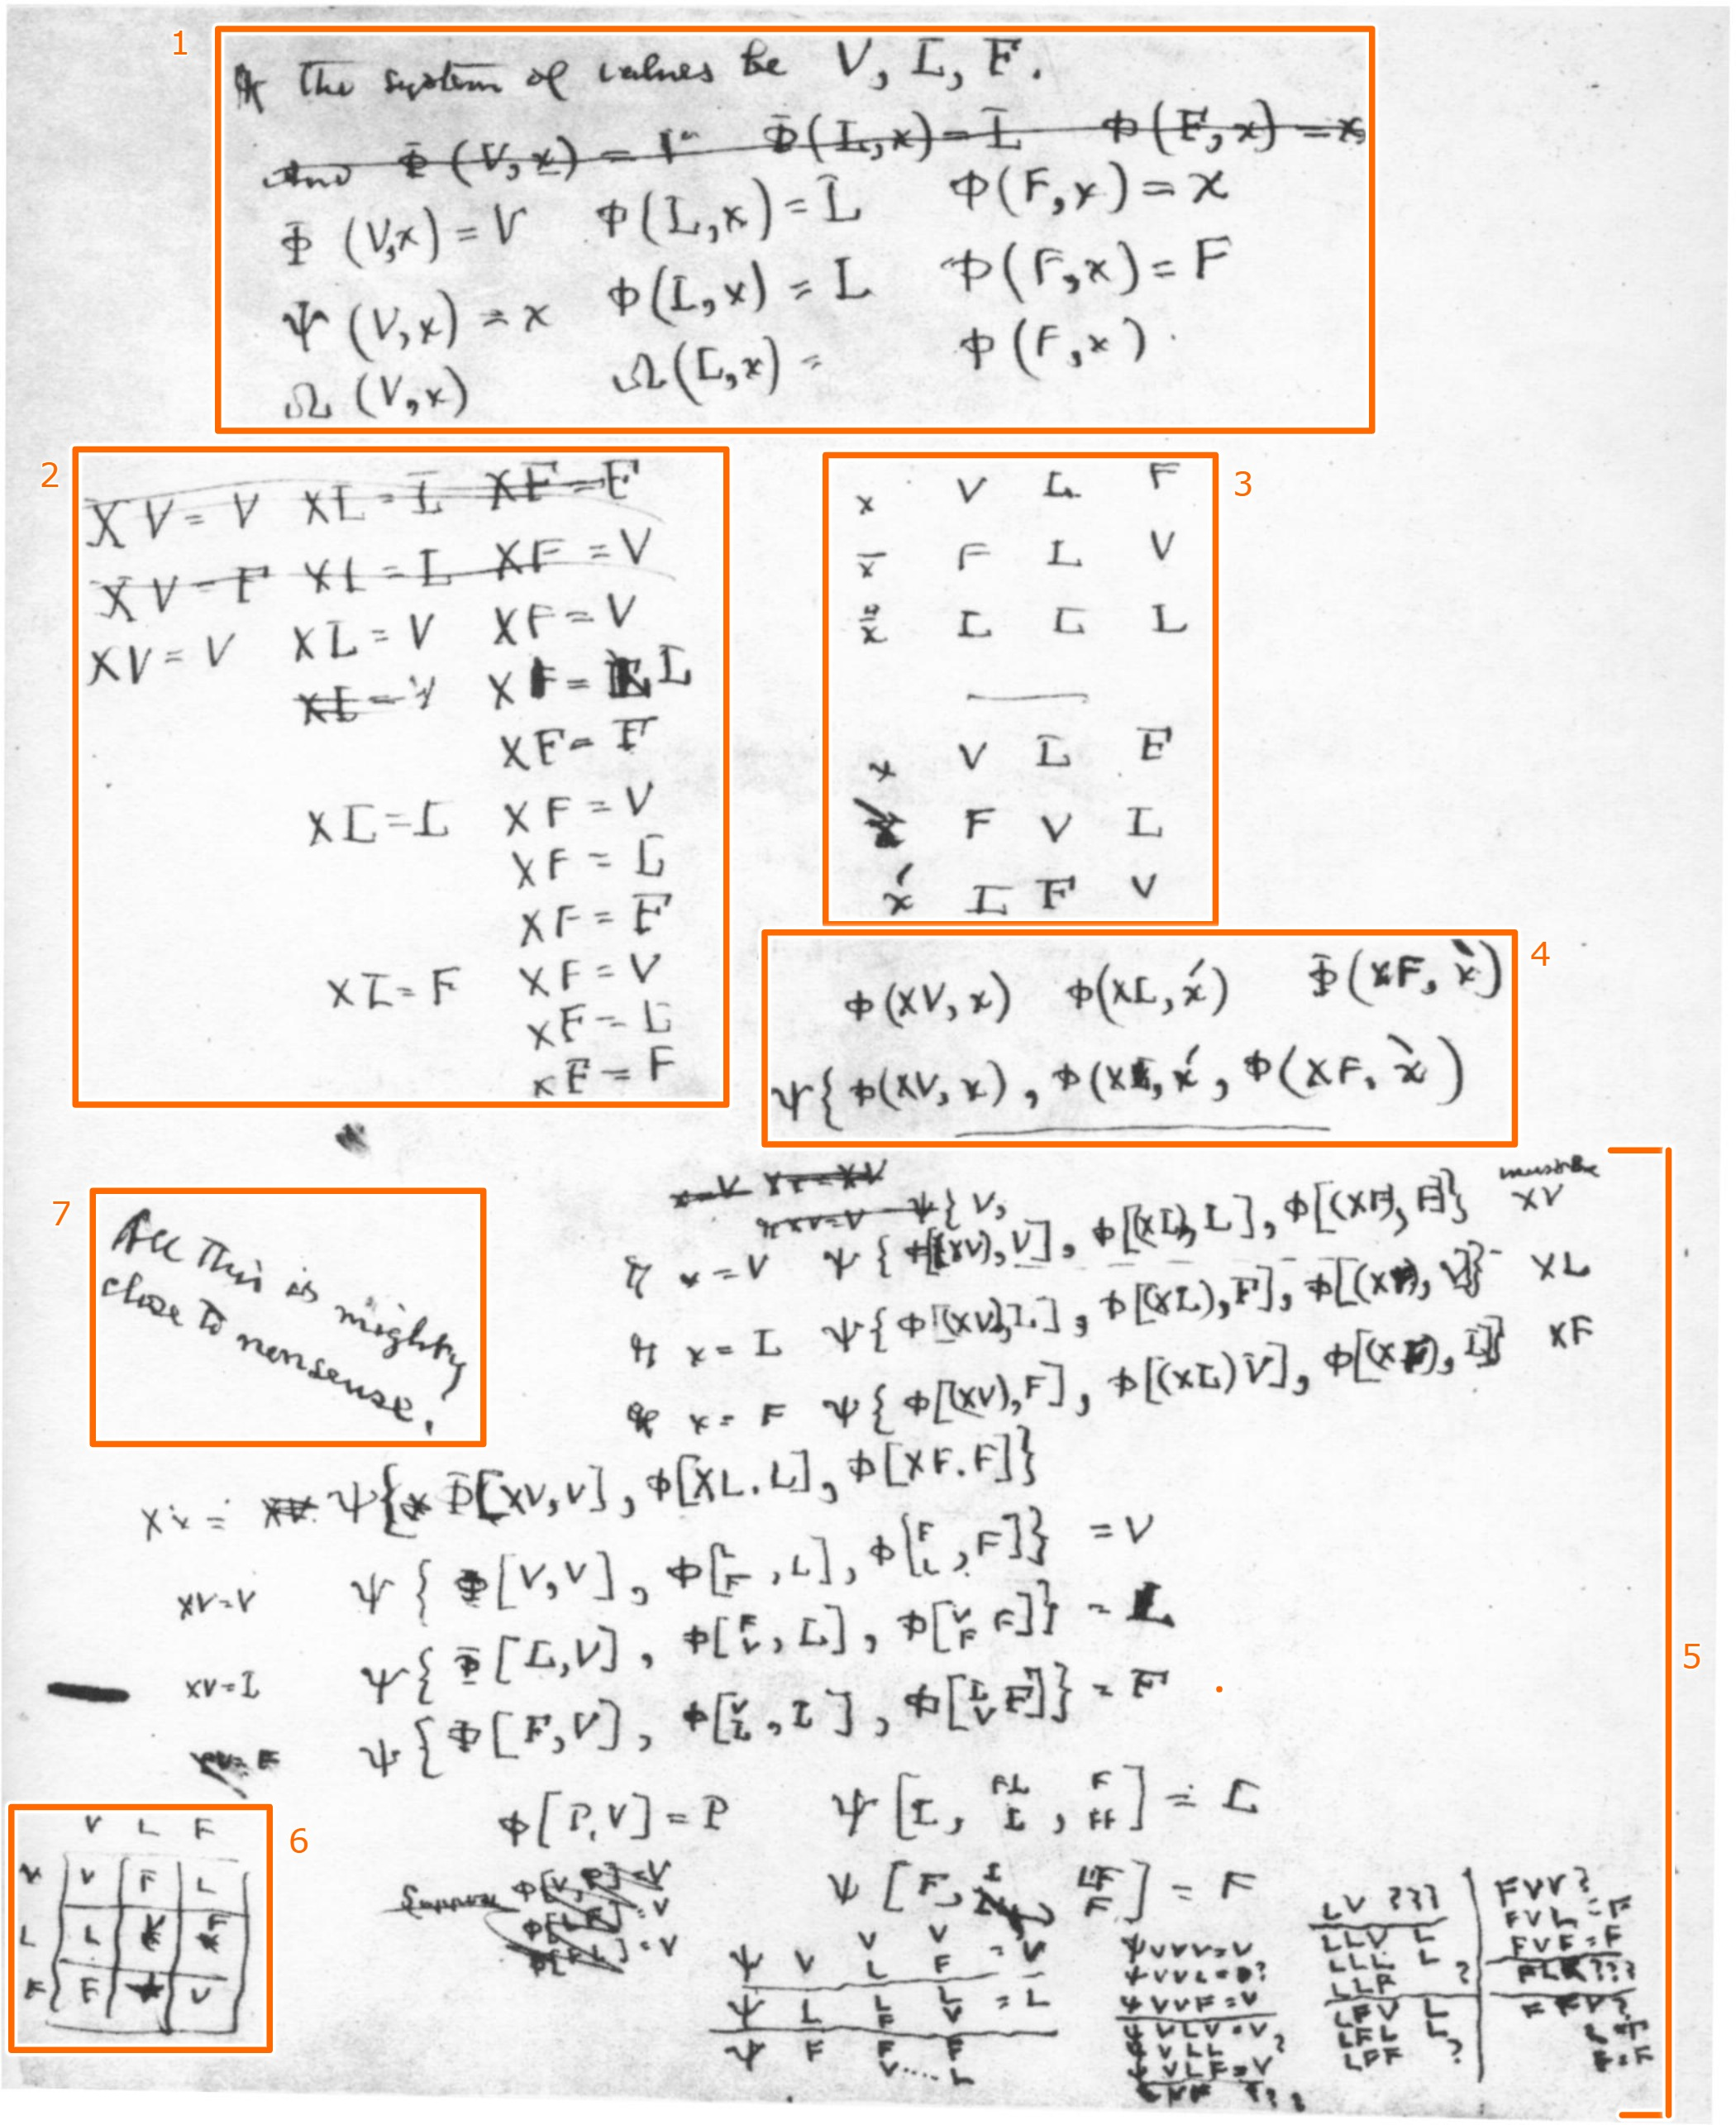
\includegraphics[width=\textwidth]{images/page one.jpeg}
    \caption{First Page, \href{https://iiif.lib.harvard.edu/manifests/view/drs:15255301$638i}{seq. 638 V.}}
    \label{fig:seq638}
\end{figure}



The first page begins (1) ``Let$[\!\![$?$]\!\!]$\footnote{There are times when Peirce's writing is illegible, reducing confidence in the accuracy of my transcriptions. In these cases I will put a `?' in double square braces to indicate the possibility of error. When these marks appear without the braces they are part of the original manuscript.} the system of values be $V, L, F$.'' The first line is crossed out and appears to have read ``And $ \Phi(V,x)=F$[\!\![$?$]\!\!]$ \enspace \Phi(L,x)=L	\enspace	\Phi(F,x)=x$.'' The first definitions are for the $\Phi$, $\Psi$, and $\Omega$ operators.
\begin{gather*}
\Phi(V, x)= V, \enspace \Phi(L,x)=L, \enspace \Phi(F, x)=x\\
\Psi(V,x)=x, \enspace \Phi(L, x)=L, \enspace \Phi(F,x)=F\\
\Omega(V,x), \quad \Omega(L,x)=\enspace, \quad \Phi(F,x)
\end{gather*}
Presumably the $x$ in these formula can take any value, so the first formula of the top line should be read as `phi of a \textit{verum} proposition and any proposition is \textit{verum}.' Peirce seems to have been focused mainly on defining the $\Phi$ operator on this page. The crossed out line conflicts with the first formula of the top line. The middle line conflicts with the top in the third formula, but it agrees with the crossed out first line in this regard. These disagreements seem to indicate a certain amount of indecision on Peirce's part and it is difficult to tell what kind of connective he wanted $\Phi$ to be. The middle line also introduces the $\Psi$ operator, but only provides one valuation for it. The third line introduces $\Omega$ but does not give any valuations for the formulae on it.

Immediately below on the left (2), there appears to be some scratch work made in an attempt to define a one place operator $X$\footnote{It is typographically difficult to make clear, but this character is meant to be the greek letter Chi.}. The valuations are sorted into three columns based on whether $X$ is operating on $V, L,$ or $F$. Peirce seems to have confidence that $XV=V$, but waffled over the value of $X$ of $L$ and $F$. In the second and third columns he has listed all the possible valuations for when $X$ is applied to $L$ or $F$. He may have just wanted to write all of the combinations down to keep track of the possibilities. Another possible interpretation is that these equations were shorthand for combinations and valuations of $\Phi$, $\Psi$, or $\Omega$ formulae. The issue with this interpretation is that on other pages (seq.639 and 641), $X$ is clearly a unary operator.

To the right (3) appears to be the only part of the first page deemed worth salvaging. Here Peirce defines four unary operators. $\bar{\lnot}x$\footnote{While Peirce uses different accents to symbolize his various negations, like $\bar{x}$, $\mathring{\bar{x}}$, $\acute{x}$, and $\grave{x}$, I have elected to use prefix operators, $\bar{\lnot}x$,  $\mathring{\bar{\lnot}}x$, $\diagdown{x}$, and $\diagup{x}$, instead.} appears to be the standard interpretation of negation in three valued logic and is common to Łukasiewicz's system. $\mathring{\bar{\lnot}}x$ is the operator that gives $L$ no matter the input. It corresponds to Slupecki's ``tertium function" \citeyearpar{slupecki_volle_1937} and could be used as a constant of sorts. (It may also be possible to define modal functors with $\mathring{\bar{\lnot}}x$.) $\diagdown{x}$ and $\diagup{x}$ match up with two negations that Post defines in his system. These negations turn out to be rather important for Turquette when he shows that Peirce's semantics are functionally complete and when he extends this system into a sound and complete logic. Out of the four unary operators on the page, only $\diagdown{x}$ and $\diagup{x}$ are what Turquette calls total negations. This is because out of the four they are the only ones that transform all of the values for whatever they are applied to. $\bar{\lnot}x$ and $\mathring{\bar{\lnot}}x$ only transform two of the values and keep $L$ the same. $\diagdown{x}$ and $\diagup{x}$ have an oddly cyclical nature. Notice that $\diagdown{}(\diagdown{}(\diagdown{x}))=x=\diagup{}(\diagup{}(\diagup{x})$. \footnote{Perhaps there is some connection with the cyclical arithmetic that Peirce discusses in his ``Amazing Mazes'' articles in \textit{The Monist} written around the same time \citep{peirce_amazing_1908}.}

\begin{displaymath}
\begin{array}{|c|c|c|c|c|}
% |c c|c| means that there are three columns in the table and
% a vertical bar ’|’ will be printed on the left and right borders,
% and between the second and the third columns.
% The letter ’c’ means the value will be centered within the column,
% letter ’l’, left-aligned, and ’r’, right-aligned.
p & \bar{\lnot}x & \diagdown{p} & \diagup{p} & \mathring{\bar{\lnot}}p\\ % Use & to separate the columns
\hline % Put a horizontal line between the table header and the rest.
V & F & F & L & L\\
L & L & V & F & L\\
F & V & L & V & L\\
\end{array}
\end{displaymath}

Immediately below the unary operators (4), Peirce appears to be experimenting with $\Phi$, $\Psi$ and the two cyclical negations. The other more mysterious unary operator, $X$, also features in these formulae. It is unclear what the point of this was.

Little can be gleaned from the area (5) immediately below either since it is not clear what $XV, XL,$ or $XF$ express unless they somehow match up with the work done in (2). This seems unlikely though because the values on any combination other than $XV$ in (2) are ill defined. He seems to have been trying to work out $\Psi$ however, here it appears as a three place operator. Its being considered as a three place operator is demonstrated by the array on the bottom right of the page and by its taking of three $\Phi$ formulae as arguments above this. However, these would still make sense if $\Psi$ was a two place operator, as long as it was associative.

On the bottom left of the page (6) there is a characteristic matrix for some undisclosed operator. It does not to match up with any of the completed matrices that appear on the next page under discussion, seq. 640.

In the middle of the left (7) we find what is perhaps Peirce's admission of defeat. The text reads ``all this is mighty close to nonsense." It seems he was ultimately unsatisfied with the work done on this page. His primary concern here seems to be working out definitions for $\Phi$ and $\Psi$ and possibly some relationship between the two, as shown by the nesting of $\Phi$ formulae within $\Psi$ formulae. Since the Post negations also feature in some of these formulae, its possible that they played a role in this relationship.

\section{seq. 640 V.}

\begin{figure}
    \centering
    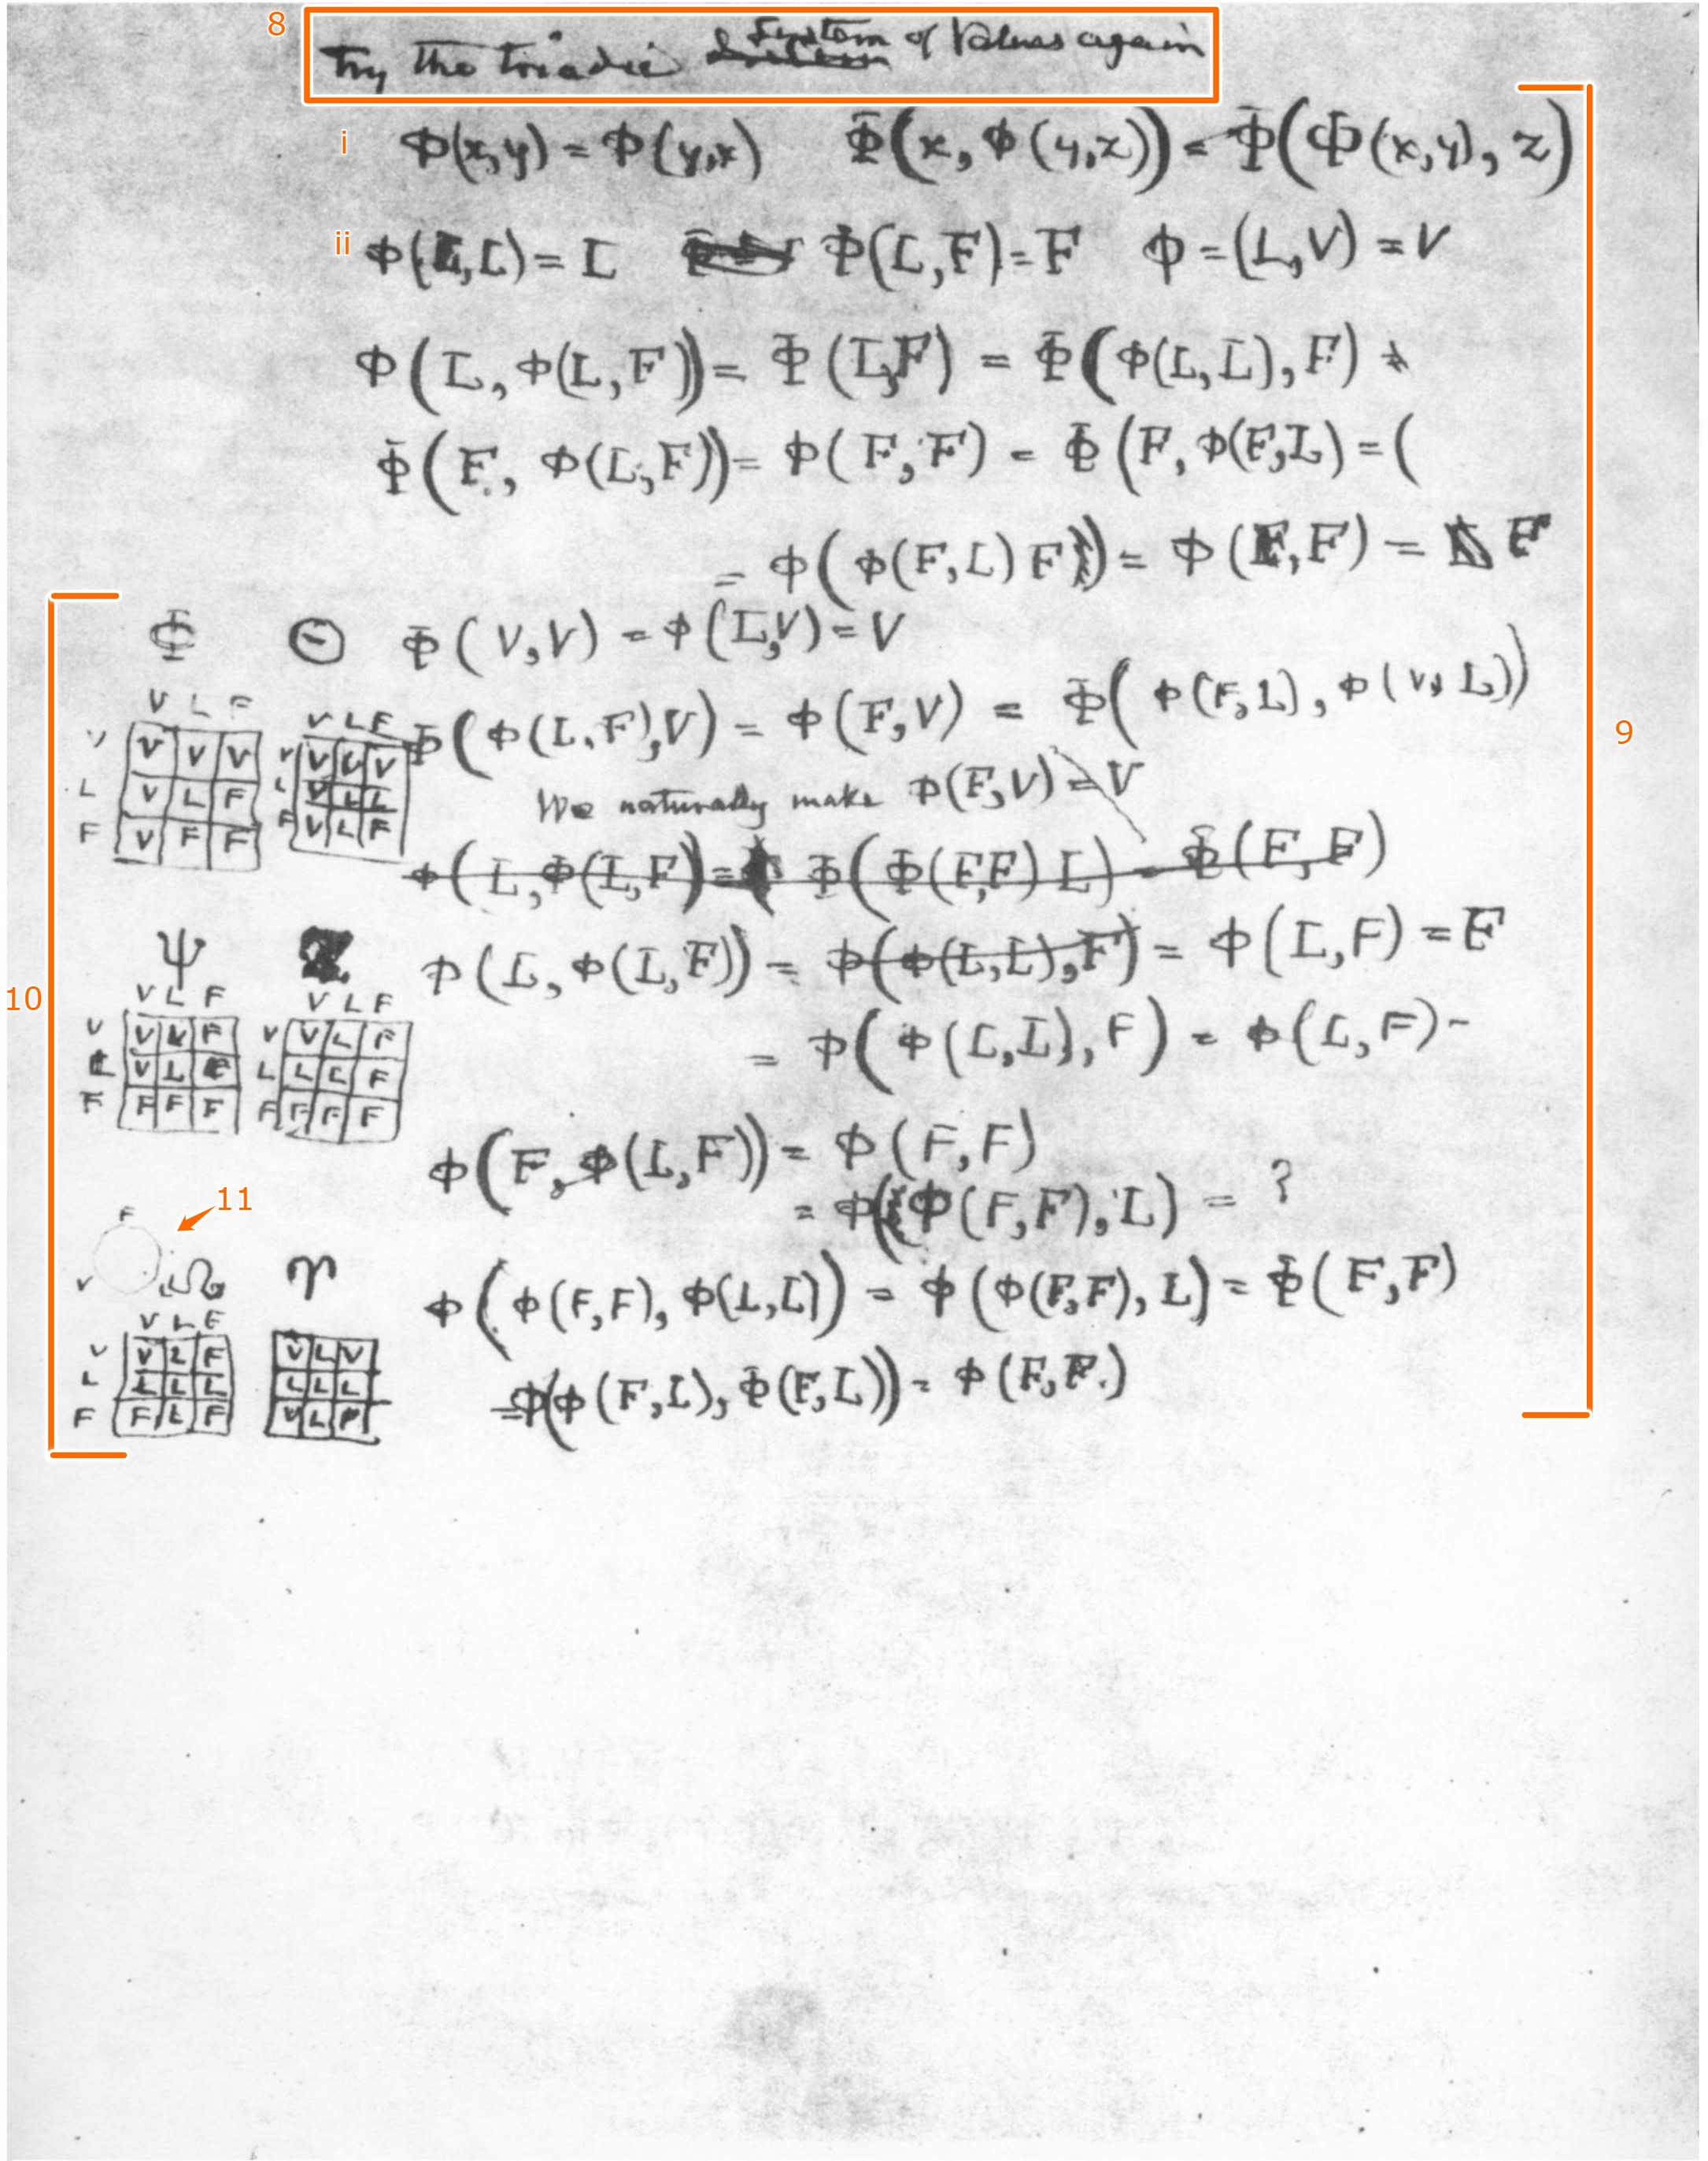
\includegraphics[width=\textwidth]{images/page two.jpeg}
    \caption{Second Page, \href{https://iiif.lib.harvard.edu/manifests/view/drs:15255301$640i}{seq. 640 V.}}
    \label{fig:640}
\end{figure}

The second page appears to have been far more successful. At the top of the page (8) is written ``try the triadic system of values again.'' Below the word `system', `definition' appears crossed out.

The bulk of the page (9) appears to be devoted to working out the semantics of $\Phi$. On the first line (i) two formulae appear, indicating that $\Phi$ is both commutative and associative. Line two (ii) gives valuations for $\Phi$ when paired with $L$ and any value. In lines 3, 4, and 5, the formulae in (ii) are slotted in either place of $\Phi$ and are identified with other combinations. The rest of (9) amounts to more of the same. Given that all that Peirce had worked out for $\Phi$ in the main body of the page is consistent with its characteristic matrix on the left, it seems reasonable to conclude that the main goal here was to give this definition. It seems he was successful in these regards as well.
\begin{displaymath}
\begin{array}{|c c|c|c|}
% |c c|c| means that there are three columns in the table and
% a vertical bar ’|’ will be printed on the left and right borders,
% and between the second and the third columns.
% The letter ’c’ means the value will be centered within the column,
% letter ’l’, left-aligned, and ’r’, right-aligned.
p & q & \Phi(p, q) & \Psi(p, q)\\ % Use & to separate the columns
\hline % Put a horizontal line between the table header and the rest.
V & V & V & V\\
V & L & V & V\\
V & F & V & F\\
L & V & V & V\\
L & L & L & L\\
L & F & F & F\\
F & V & V & F\\
F & L & F & F\\
F & F & F & F\\
\end{array}
\end{displaymath}

One curiosity resulting from this is that in the marginal note (10) we find not one, but six operators with characteristic matrices. It is not immediately clear where all of the other operators came from. While it is certainly possible that he had worked these out on other pages that have since been lost, it is also possible that one operator was all he needed to work out the others. This would not be totally uncharacteristic of Peirce as he had earlier shown, in MS 378, that all boolean operators could be built up from combining $\lnot$ and $\lor$ into a single logical operator, which we now call `nor' (CP 4.12-20, from an untitled paper written in 1880). So, it seems possible that once he had a consistent definition of $\Phi$ worked out, he was able to discover the rest of the operators by combining $\Phi$ with the negations he worked out on the previous page. This idea is somewhat supported by the complex network of morphisms between the operators that Turquette discovered \citep{turquette_dualism_1972}. Every one of Peirce's operators is the dual of some other with respect to the $\bar{\lnot}x$ negation ---where an operator $O$ is the dual of another $O^{*}$ with repect to a negation $\lnot^{i}$ just in case $\lnot^{i}(\lnot^{i}p O \lnot^{i}q)\equiv (p O^{*} q)$--- like $\land$ and $\lor$ in classical logic. For example, $\Phi$ is the dual of the $\Psi$ operator immediately below it with respect to $\bar{\lnot}x$. In the same fashion, $\Theta$ and $Z$ are duals, and so are $\Omega$ and $\Upsilon$. 

Another layer of depth in this network of relations can be appreciated if we consider the cyclical total negations Peirce gave on the first page. For any one of the operators on the page there is a tri-morphism ---where an operator $O$ has $O^{*}$ and $O^{'}$ as trimorphs with respect to a cyclical negation $\mathring{\lnot}$ just in case $(pOq\equiv \mathring{\lnot}(\mathring{\lnot}pO^{*}\mathring{\lnot}q))\land (pOq\equiv \mathring{\lnot}\mathring{\lnot}(\mathring{\lnot}\mathring{\lnot}pO^{'}\mathring{\lnot}\mathring{\lnot}q))$ holds between $O$ and the other two operators. For example $p\Phi q$ is equivalent to both $\diagdown{}(\diagdown{p}Z\diagdown{q})$--- and $\diagup{}(\diagup{p}\Upsilon \diagup{q})$. It turns out that in the six operators defined in the margin, there are two trimorphisms. While $\Phi, Z$ and $\Upsilon$ are trimorphs of each other, so are $\Psi, \Theta$ and $\Omega$.

There is some textual evidence Turquette points out to support the idea that Peirce was aware of this relationship \citep{turquette_dualism_1972}. If we look closely to the left of $\Omega$ (11), there appears to be a small circle with $V, L$ and $F$ around the perimeter about 120 degrees apart from one another. Moving clockwise around the circle appears to correspond with the $\diagdown{x}$ negation ($\diagdown{V}=F, \diagdown{F}=L,$ and $\diagdown{L}=V$). Moving counterclockwise corresponds to the $\diagup{x}$ negation ($\diagup{V}=L, \diagup{L}=F,$ and $\diagup{L}=V$). This may suggest, as Turquette claims, that Peirce was aware of these trimorphisms and was experimenting with his cyclical negations while developing his operators.

Even more dualisms can be found if we consider negations other than the ones Peirce gave, as Turquette has also shown. However, restricting ourselves only t0 the negations Peirce treated in these notes, we can draw the following network of relations between his operators:


% https://tikzcd.yichuanshen.de/#N4Igdg9gJgpgziAXAbVABwnAlgFyxMJZABgBpiBdUkANwEMAbAVxiRAB12AFACyxAC+pdJlz5CKAEzkqtRizacAKjxg46g4SAzY8BImQCMs+s1aIO3bJpG7xRaceqmFFgFo3tovRJKlJJvLmlgDyALYwAOYaQrZi+lL+gWaK7ACqaNgM+gKyMFCR8ESgAGYAThBhSGQgOBBI0iAMdABGMAxc3vYWWGDYsCDOQaktdGXAAB4CgyCqdFBskGCs1HB8JTjV1Ay9wXAQOwvU6lgMiwQrIG1gC4jEsSDllUiGx-WIAMxDKRaco+NTGZzW7gC4zZptDpdBIgXr9S7XW73LRPKqIAAsbyQAFZvq5LP9JtNtq12p07DC4VgBtRgedljNEdUHqitrV3l85D9LJEynQaDAieDSVCKRImjANoyYDdmSiKmjOXUcSTIeT4uKGJLNnjgpxefzBYDqEy7iyFSr2WyXHr2AaBULVWToeKylhIjwdVcZUjzc9EK8rYhGhDnWK2G6PV7TTUbal7Ubpn60Y1lRjdfG+Q7jU0ReqfBH3Z7PKz00HA6HRRq2FqpRnfnas4nBBQBEA
\[
\begin{tikzcd}
\Phi \arrow[d, "\bar{x}" description, no head] \arrow[rrd, "\diagdown{x}"]     &  & \Theta \arrow[d, "\bar{x}" description, no head] \arrow[lld, "\diagdown{x}"'] \\
\Psi \arrow[d, "\diagdown{x}"']                                                &  & Z \arrow[d, "\diagdown{x}"]                                                   \\
\Omega \arrow[rr, "\bar{x}" description, no head] \arrow[rruu, "\diagdown{x}"] &  & \Upsilon \arrow[lluu, "\diagdown{x}"']                                       
\end{tikzcd}
%\begin{tikzcd}[row sep=large,column sep=large]
%\Phi \arrow[d, ''\bar{x}'' description, no head] \arrow[rrd, ''\diagdown{x}'']     &  & \Theta \arrow[d, ''\bar{x}'' description, no head] \arrow[lld, ''\diagdown{x}'''] \\
%\Psi \arrow[d, ''\diagdown{x}''']                                                &  & Z \arrow[d, ''\diagdown{x}'']                                                   \\
%\Omega \arrow[rr, ''\bar{x}'' description, no head] \arrow[rruu, ''\diagdown{x}''] &  & \Upsilon \arrow[lluu, ''\diagdown{x}''']                                       \end{tikzcd}
\]
In the diagram the lines without arrowheads that are separated by $\bar{\lnot}x$ in the middle mark the dualisms. The directional arrows mark the $\diagdown{x}$ trimorphisms. If the direction of the arrows is reversed the $\diagup{x}$ trimorphisms can be observed. These considerations may offer a possible explanation for how Peirce got the full set of operators after seemingly only defining $\Phi$. For example, from $\Phi$ he could have worked out its $\bar{\lnot}x$ dual, $\Psi$. From there he could have worked the rest out by applying either $\diagdown{x}$ or $\diagup{x}$ to these two to unveil each of their trimorphs.\footnote{For further discussion on the relationships between Peirce's triadic operators and to see how they can be used to make a sound and complete logic under different axiom sets and with the addition of quantification, see \cite{turquette_peirces_1967, turquette_storrs_1968, turquette_peirces_1969, turquette_minimal_1976, turquette_alternative_1978, turquette_quantification_1981, turquette_defining_1988}} However, the textual evidence is so small that concluding as such would be a bit of a leap.

Each of Peirce's operators also has an analogue in more familiar modern systems of three-valued logic. The most familiar of these are $Z$ and $\Theta$, which are the versions of conjunction and disjunction in Łukasiewicz's system as well as Kleene's strong conjunction and disjunction (\citeyear{kleene_introduction_1952}, 327-336). $\Upsilon$ corresponds to a connective used by Bochvar as well as Kleene's weak disjunction \citep{bochvar_three_1939}. Likewise, $\Omega$ corresponds to another of Bochvar's connectives and Kleene's weak conjunction. $\Phi$ and $\Psi$ are probably the most obscure of these operators. They appear as disjunction and conjunction respectively in a system developed by Sobocinski \citeyearpar{sobocinski_axiomatization_1952} as well as in Coopers ``logic of ordinary discourse'' \citeyearpar{cooper_propositional_1968} which was pointed out by R. Z. Parks \citeyearpar{parks_mystery_1971}.\footnote{For more connections between Peirce's three-valued operators and more recent works, see \cite{lane_2001}.}

It may also be worth noting that Turquette has proven that any one of Peirce's operators along with either one of the cyclical negations can form an expressively complete system. Extrapolating on this work further to suggest what Peirce's definition of implication, Turquette was also able to develop a sound and complete axiomatic system of three-valued propositional logic with one inference rule.
%maybe watch video. it's going to take a few more sentences here.

Another interesting curiosity is that all of Peirce's operators seem to be versions of conjunctions and disjunctions, and he seems to have shown little interest in asymmetric relations, like conditionals. So, why was Peirce so preoccupied with these kinds of operators? This possibly has to do with the kinds of things he was hoping to represent within this system. It is also possible that he was not sure how he wished to define a conditional operator for his triadic logic. This doesn't seem to have stopped him with regard to conjunction or disjunction, as he appeared to be content to have multiple forms of these.

\section{seq. 645 R.}

\begin{figure}
    \centering
    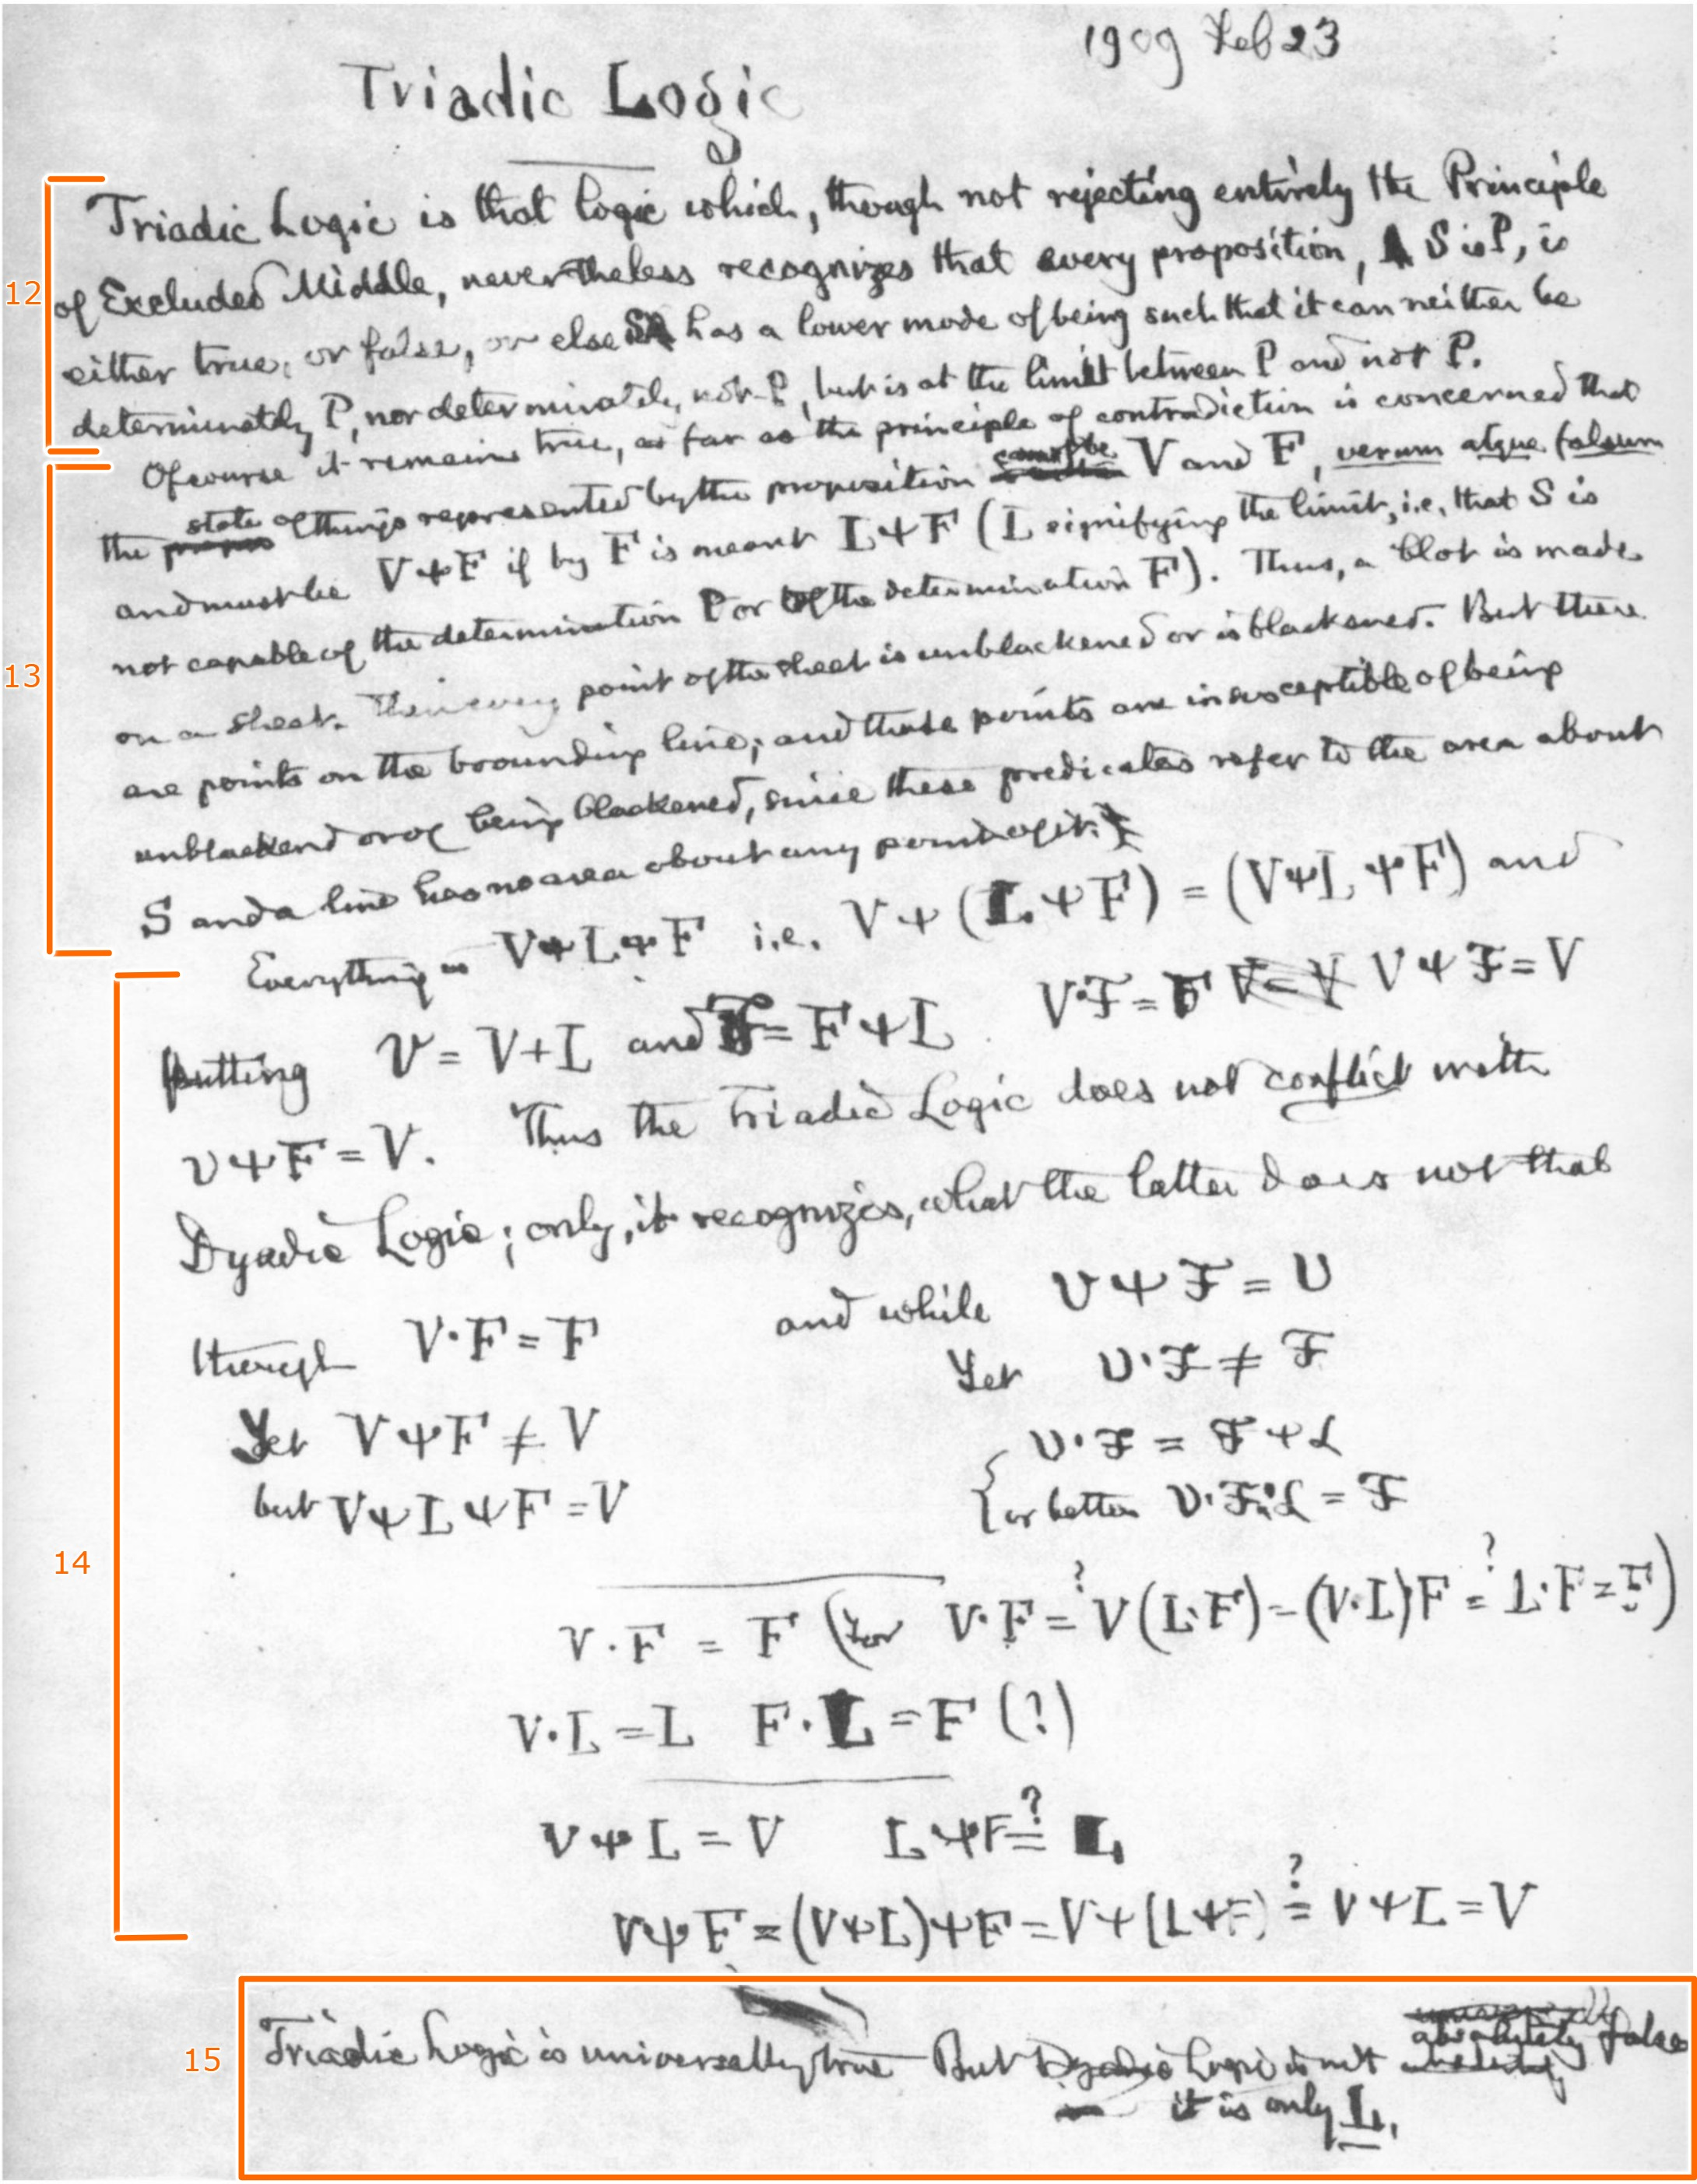
\includegraphics[width=\textwidth]{images/page three.jpeg}
    \caption{Third Page, \href{https://iiif.lib.harvard.edu/manifests/view/drs:15255301$645i}{seq. 645 R.}}
    \label{fig:645}
\end{figure}

The third and final page is the most substantive in terms of textual evidence for exactly what Peirce was trying to accomplish with his three-valued semantics. In it we find a description of triadic logic along with a rather bizarre example of the sorts of things he intended $L$ to apply to. The page is titled ``Triadic Logic'' and is dated February 23, 1909. 

The text (12) begins: \begin{quotation}\noindent``Triadic logic is that logic which, though not rejecting entirely the principle of excluded middle, nevertheless recognizes that every proposition, S is P, is either true or false, or else S has a lower mode of being such that it can neither be determinately P, nor determinately not P, but is at the limit between P and not P.''\end{quotation} This passage will be important for my later analysis. He does not mention here what he means by `mode of being' but this notion figures importantly in his philosophy elsewhere. To explain this notion requires a brief foray into an aspect of Peirce's thought I have referred to as his triadism: his penchant for making tripartite divisions in philosophy.  Peirce developed a concept of three Universal\footnote{He seems to have thought of these categories as being of higher order than even metaphysical categories.} Categories that he used in his analysis of all philosophical ideas. He sometimes calls them categories of being, sometimes of ideas, of thoughts, and of nature (or `things' as he usually says). Depending on the subject matter, these categories will have different names, but in the most abstract sense they are always the same. In his 1904 letters to Lady Welby, he defines these categories as follows:
\begin{quotation}
\noindent``Firstness is the mode of being of that which is such as it is, positively and without reference to anything else.

Secondness is the mode of being of that which is such as it is, with respect to a second but regardless of any third.

Thirdness is the mode of being of that which is such as it is, in bringing a second and third into relation to each other.'' (CP 8.328)
\end{quotation}
 In the abstract, the categories are firsts (things that are what they are without reference to anything else), seconds (things that exist only in reference or connection something else), and thirds (which exist in bringing together a second and a third). An example of the sort of thing that would be a first for Peirce is a quality, like a color. There is some sense in which colors exist without reference to anything else. We all have a concept of `redness' that we can think of independently of red objects. So the color red is a first. Seconds are like particular objects, like a red blanket. A red blanket is what it is in reference to two things: being red and being a blanket. Thirds do not lend themselves to simple examples as easily, and are more recognizable within the various contexts Peirce applies his categories. He sometimes calls them laws, sometimes reasons, and other times powers.

Having some idea of Peirce's categories, we can now examine his three modes of being. Each of the objects that falls into his three categories has an associated mode of being: ``My view is that there are three modes of being. I hold that we can directly observe them in elements of whatever is at any time before the mind in any way. They are the being of positive qualitative possibility, the being of actual fact, and the being of law that will govern facts in the future'' (CP 1.23). So, firsts, being merely qualities, have the mode of being of a possibility. This is because they do not exist on their own except for in the possibility that they are instantiated by some object, in the sense that the color red does not really exist independently of red objects. Seconds, have the mode of being of actuality. These are ordinary objects that occur in the world around us. All the objects that we normally see and interact with are seconds. Thirds have the mode of being of necessity. Again, this notion is much more difficult to understand as precisely as the first two. The things that are thirds for Peirce can loosely be understood as laws of nature. They are basically general facts about seconds. He says ``This mode of being which \textit{consists}, mind my word if you please, the mode of being which \textit{consists} in the fact that future facts of Secondness will take on a determinate general character, I call a Thirdness'' (CP 1.26). Part of the difficulty with understanding and stating precisely what thirds are is thinking of them as objects. We do not normally think of laws as objects. Nonetheless, suppose that every time a diamond is dragged across a pane of glass, from now into the indefinite future, a scratch is produced. Then the third in this case is the law or fact of the universe that determines that all diamonds scratch all panes of glass.

Having cleared up Peirce's categories and modes of being, it is already clear that modality was built in to these notions. When Peirce discusses triadic modality, as well as when Fisch and Turquette, Lane, and I do so, it is the possibility, actuality, and necessity built into these modes of being that we are referring to. So when Peirce refers to ``modes of being'' in his logic notebook, there is clearly some sense in which modality is involved.

The note goes on to say (13) ``Of course it remains true, as far as the principle of contradiction is concerned that the state of things represented by the proposition cannot be $V$ and $F$, \textit{verum atque falsum} and must be $V+F$ if by $F$ is meant $L+F$ ($L$ signifying the limit, i.e. that S is not capable of the determination P or of the determination $F$).''\footnote{When Peirce uses $+$ in this way, it is just a notational variant of $\lor$.} Peirce's strange example then follows: ``Thus, a blot is made on a sheet. Then every point of the sheet is unblackened or blackened. But there are points on the boundary line; and those points are insusceptible of being blackened or of being unblackened, since these predicates refer to the area about S and a line has no area about any point of it.'' 

At first glance this seems to be an example of a category mistake. The proposition `point $x$ on the boundary line is blackened' should apparently take the value $L$, because $x$ would have to have area in order to be blackened or unblackened, and points on lines do not have area. Thus, this predicate is undefined for $x$. The strange thing is that points themselves do not have any area, which runs contrary to Peirce's claim that ``every point of the sheet is blackened or unblackened.'' Another possible interpretation is that he thought that the properties of a point were determined by the properties of the immediate area surrounding the point. This view would make more sense, as the points on the boundary line really would be neither fully blackened nor unblackened, because the immediate area surrounding them would be both. But it is unclear from this passage alone whether this interpretation is accurate. At face value, it is also unclear how this example is supposed to relate to Peirce's earlier comment about modes of being. As far as examples go, this one is not very enlightening. It turns out that the example actually pertains to Peirce's theory of continuity, as Lane argues \citeyearpar{lane_peirces_1999}. 

The bulk of the rest of the page (14) contain Peirce's metalogical observations about triadic logic and traditional two valued logic. The sentence in the middle reads ``Thus the triadic logic does not conflict with dyadic logic; only it recognizes what the latter does not, that though...'' and then he uses formulae to demonstrate this lack of conflict.

At the bottom of the page (15) we find Peirce triumphantly declaring ``Triadic logic is universally true. But Dyadic Logic is not absolutely false, it is only $L$.'' So it seems Peirce was trying to extend dyadic logic rather than completely revise it.

\section{seq. 637 R.}

\begin{figure}
\centering
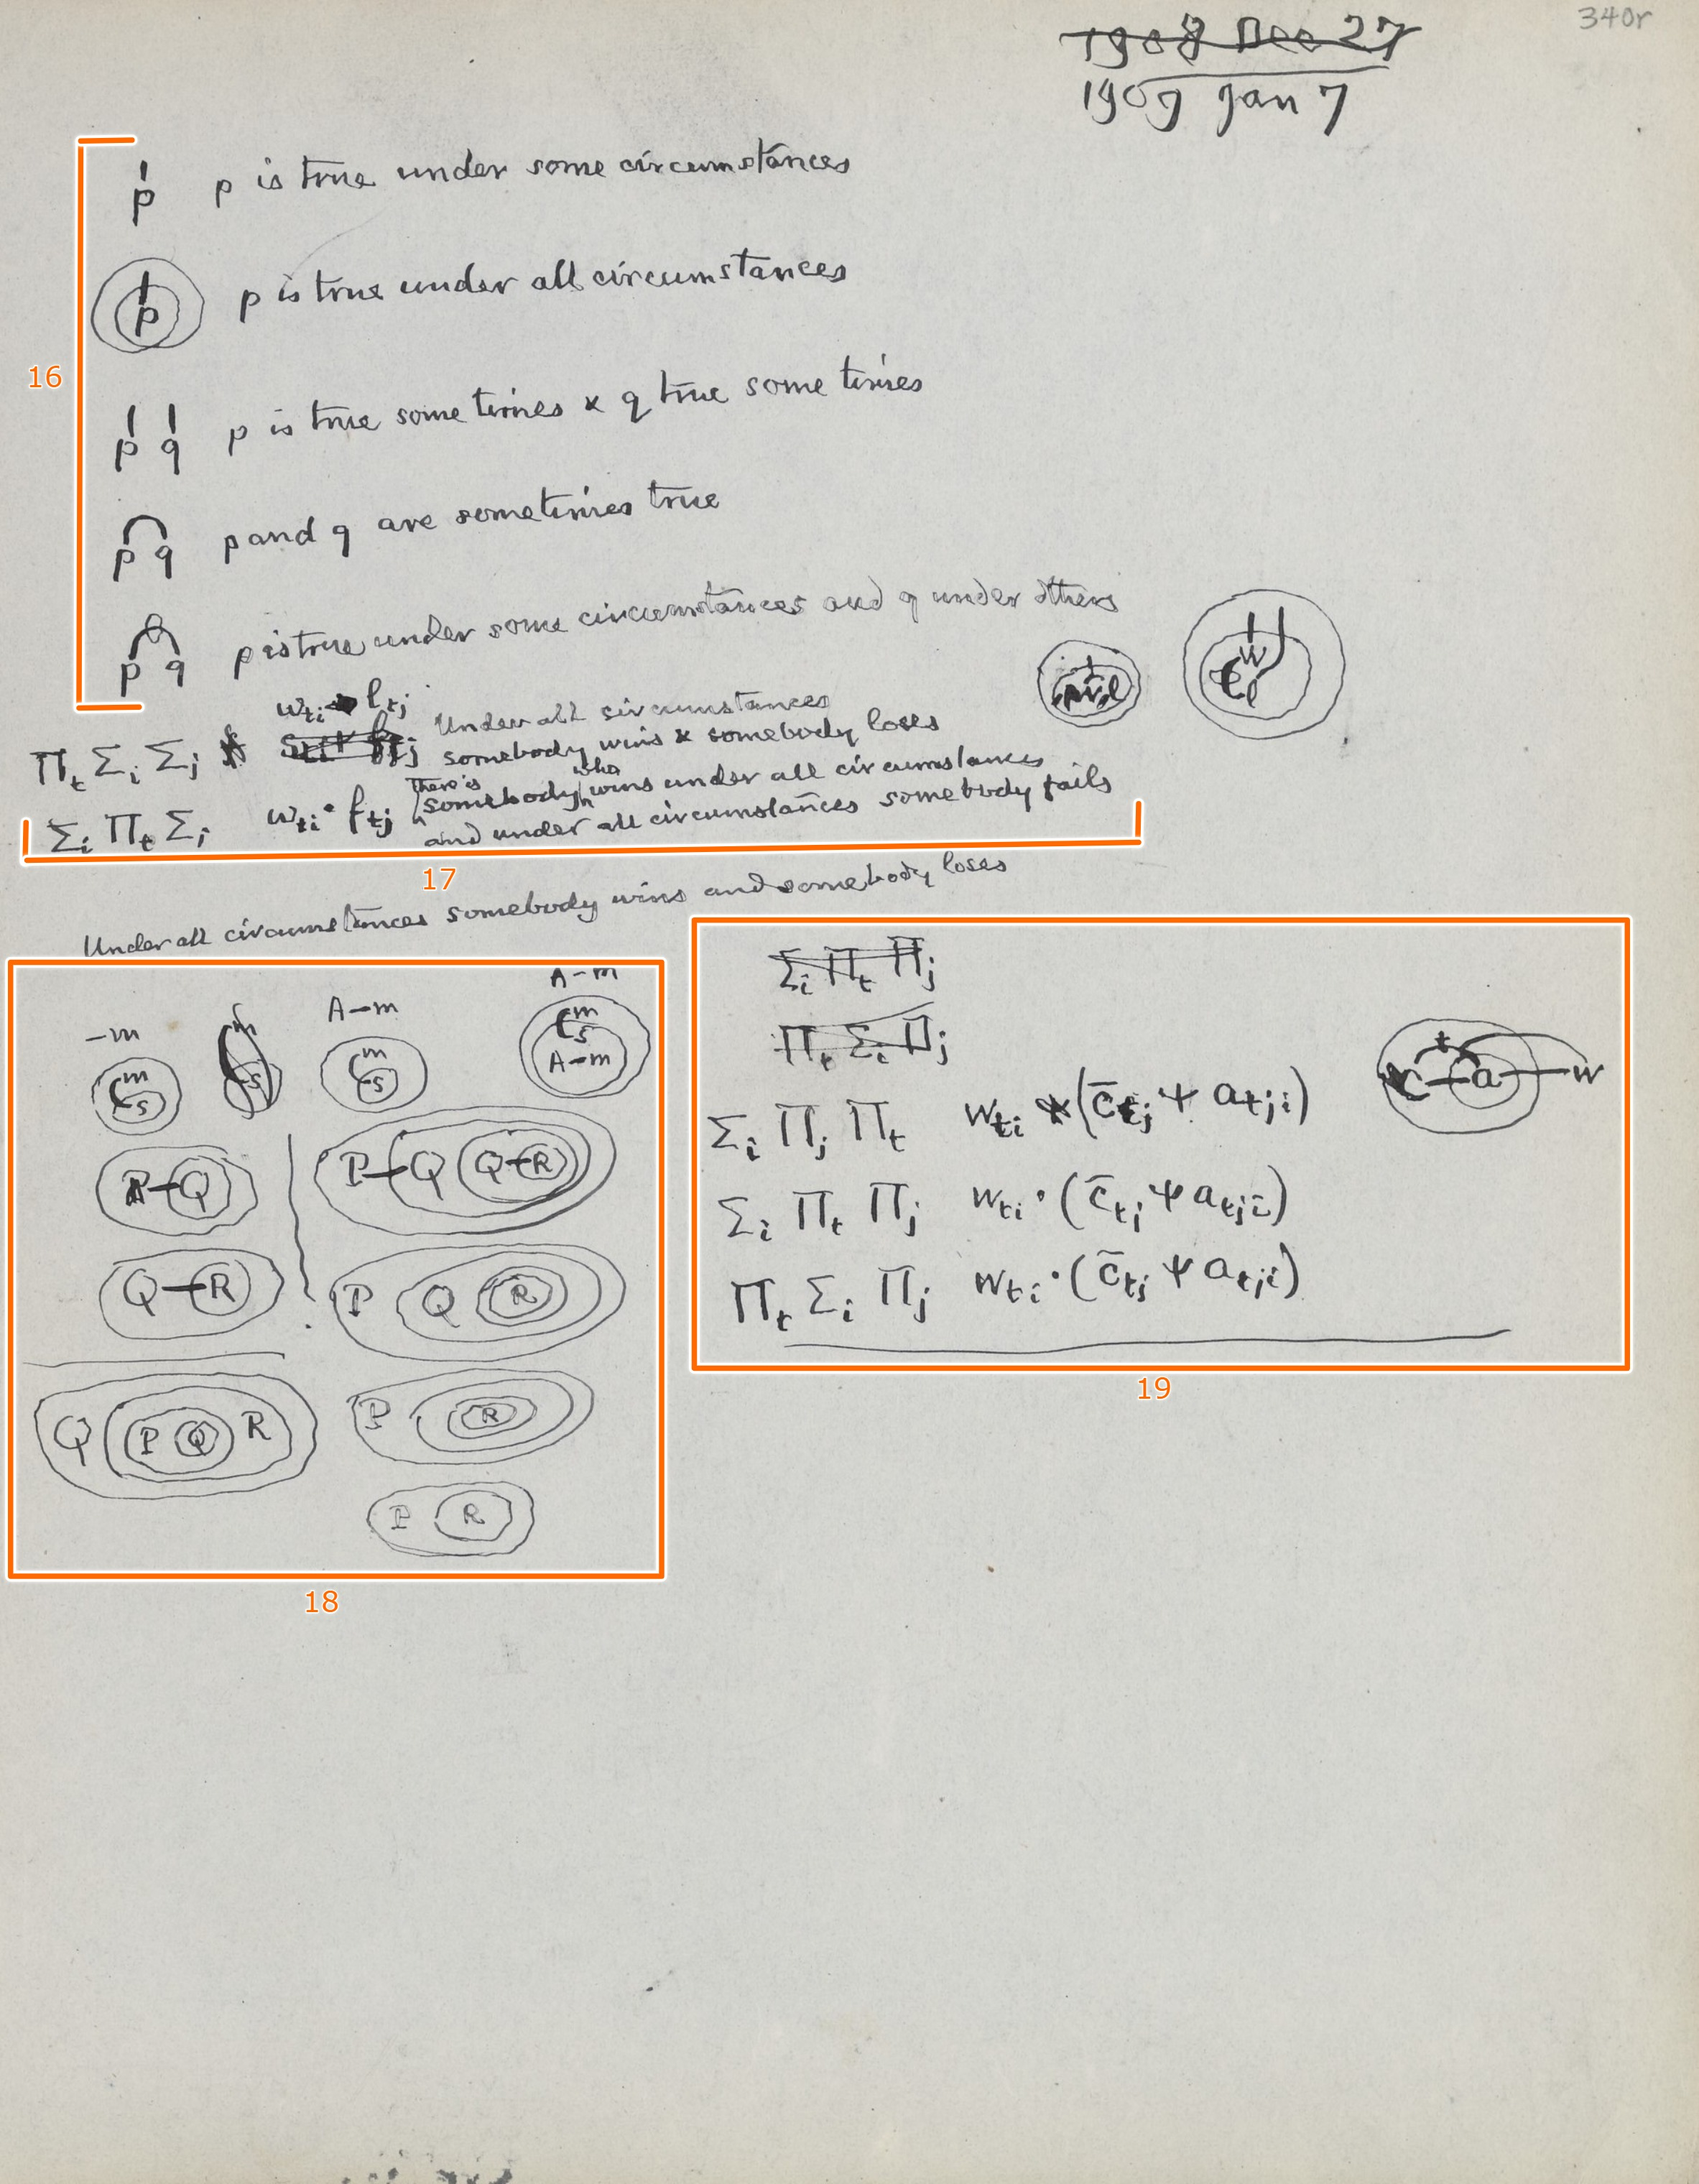
\includegraphics[width=\textwidth]{images/seq637.jpeg}
\caption{seq. 637 R.}
\label{fig:seq637}
\end{figure}

The first page preceding those that Fisch and Turquette take note of might also have some close philosophical connections to Peirce's triadic logic. In it, Peirce appears to be attempting to introduce some kind of modal operator to his already established system of existential graphs.\footnote{Peirce's discussion of existential graphs can be found in CP 4.347--584. See also \cite{roberts_existential_2009}, \cite{shin_iconic_2002}, and \cite{hammer_semantics_1998}.} Not all of the material on this page is expressed in existential graphs. On the same page, Peirce also uses algebraic notation. Fisch and Turquette do mention this page in their discussion but they tell us nothing of what is on it except that the December 27th, 1908 date has been crossed out and replaced with January 7th, 1909.

 The operator Peirce is introducing is a vertical line attached to a proposition $p$. When it is fixed to an atomic proposition, $p$, it asserts (16) ``$p$ is true under some circumstances.'' Thus, the dash appearing above $p$ on the page seems to be roughly analogous to the usual modal operator $\Diamond$. The next line shows us how to use this operator to say that a proposition is necessary. The graph to the left of this line can be translated as $\lnot \Diamond \lnot p$.\footnote{ Peirce's existential graphs are expressed using only two or three operations as long as the system is propositional or first order. For propositional logic, a closed curve indicates its contents are being negated and the juxtaposition of two formulae together indicates conjunction. For the first order system the only addition is the line of identity which operates on formulae as an existential quantifier does. Interestingly though, there were systems that were designed to treat modal propositions as well as higher order propositions. These included additional operators.} In the next line Peirce show us how to symbolize ``$p$ is true sometimes and $q$ is true sometimes.'' The lines above $p$ and $q$ in the last example can be joined to assert the conjunction of $p$ and $q$ is possible: ``$p$ and $q$ are sometimes true.'' When the joined line has an ellipse running through it, this means ``$p$ is true under some circumstances and $q$ under others.'' This would presumably mean something similar to the modal formula, $\Diamond \lnot (p \land q)$.
 
 Immediately below (17), Peirce has written some first order formulae and the English sentences these are meant to symbolize. He uses $\Pi$ and $\Sigma$ as symbols for universal and existential quantification respectively. This is nothing new as he had been using these symbols since at least 1885 when he published a paper about adding quantifiers to the already familiar set of Boolean operators \citep{peirce_algebra_1880}. The subscripts attached to the quantifiers are the variables to which they are bound. It is unclear what the connective in the first formula is but it appears to be a crossed out $\Psi$. The formula is $\Pi_{t} \Sigma_{i} \Sigma_{j} w_{ti} \xcancel{\Psi} l_{tj}$ and we are told this means ``Under all circumstances somebody wins and somebody loses.'' The next formula reads $\Sigma_{j} \Pi_{t} \Sigma_{i} w_{ti} \cdot f_{tj}$ which is interpreted as ``There is somebody who wins under all circumstances and under all circumstances somebody fails.'' For both of these formulae, the $t$ variable seems to be ranging over 'circumstances' while $i$ and $j$ range over people. Written immediately below, (17) the note says ``Under all circumstances somebody wins and somebody loses.''

Among other oddities on this page, it is unclear exactly what this example has to do with the material in the previous discussion. In the previous portion Peirce seems to be interpreting his new operator as asserting something like contingency. But there may be difficulties with this interpretation as he only states that the $p$ with a dash on top of it asserts that there are some circumstances in which $p$ is true, while contingency would require that it sometimes be false as well. This lends weight to the interpretation that regards $p$ with a dash as possible rather than contingent. A `possible' proposition would be true as long as there is at least one set of `circumstances' in which it is true. Contingency would require at least one false set as well. However, neither of these interpretations help to explain the choice of `winning,' `losing' or `failing' as an example of the kind of propositions Peirce was targeting. There is one plausible explanation though, that might lend evidence to this pages connection with Peirce's triadic logic. This is the unmentioned possibility of a `tie.' The reason Peirce may have chosen games as an example here is because there is a third possible circumstance that is often overlooked when we talk about games. This also might explain why there is no `tie' predicate on the page. If there were an additional truth value, then there would be no need for this additional predicate. The possibility of a tie would be built into the system. One might object that the second formula wouldn't make sense under this interpretation. However, that might have been the point, and this could have been a counterexample to the classical interpretation of conjunction. Another possibility is that $\cdot$ is interpreted differently in this situation, in such a way that the conjunction of middle valued statements would yield true.

At the bottom of the page, on the left (18), we can see more examples of existential graphs however the operator in the upper portion of the page makes no appearance. The lines and curves that can be observed are called ``lines of identity'' and they are used to express quantification within the system. The first three graphs from left to right in (18) involve lower case $m$ and $s$, which may refer to individuals, and an upper case $A$, which may be a predicate. Since they make no appearance in the text in the upper portions of the page, it is difficult to say how they are to be interpreted. The first graph can be translated as $\exists x m(x) \land \exists x (m(x) \lif s(x))$. The second: $\exists x(A(x) \land m(x)) \land \exists x (m(x) \lif s(x))$. The third: $\exists x (A(x) \land m(x)) \land \exists x (m(x)\lif (s(x) \land \exists y( A(y) \land m(x))))$. The rest of the graphs in this portion involve metavariables $P$, $Q$, and $R$, so Peirce probably did not have any specific interpretations in mind. One graph is boxed off from another series of graphs. The unboxed series appears to illustrate Peirce's erasure rules for his existential graphs, which are basically kinds of inference rules.

To the right (19) appears more symbolic first order formulae in which $\Psi$ makes another appearance. The `wins' predicate is involved again as well as two undisclosed predicates symbolized by `$c$' and `$a$'. A natural interpretation of `$c$' would be that it has something to do with `circumstances.' It is unclear what `$a$' is meant to be aside from a three-place predicate. The formulae are as follows:
\begin{gather*}
\Sigma_{i} \Pi_{j} \Pi_{t} w_{ti} \xcancel{\peirceor} (\bar{c}_{tj} \Psi a_{tji}) \\
 \Sigma_{i} \Pi_{t} \Pi_{j} w_{ti} \cdot (\bar{c}_{ti} \Psi a_{tij}) \\
  \Pi_{t} \Sigma_{i} \Pi_{j} w_{ti} \cdot (\bar{c}_{tj} \Psi a_{tij})
\end{gather*}
The first $\peirceor$ is crossed out presumably because Peirce meant to use the classical conjunction. Since there is no indication of what `$a$' is meant to be interpreted as, and there is no characteristic matrix given for $\Psi$ at this point, it is difficult to say what the significance of this is.

At this point I would like to raise an interesting question in connection with Peirce's existential graphs and his triadic logic. Peirce was exceedingly proud of his existential graphs, lovingly referring to them as his ``chef d'oeuvre.'' In 1903 he expressed his preference for them over his previous algebraic approach, calling them ``far more perfect'' with regards to understanding necessary reasoning (CP 4.429). Why then, if Peirce so admired and preferred his diagrammatic system, does he return to the algebraic approach when developing his triadic logic years after he was satisfied with existential graphs? His choice is odd not only because of his preference for this system but also because he had developed a system of graphs for dealing with modal propositions: the gamma graphs (CP 4.510-529 and 573-584). This may provide evidence that Peirce was not concerned with modality when developing his triadic logic, or at least not the kind of modality dealt with by his gamma graphs.

The mix of algebraic expressions and graphs on this page might be evidence that Peirce was trying to develop a graphical system capable of dealing with whatever was at issue, but that he failed to work this out to his satisfaction and reverted to his former approach. The likely explanation for this decision has to do with how logical notions like validity are given for his graphs. In the system of existential graphs (henceforth EG), deductive validity is defined syntactically according to the rules of the system, where as the algebraic approach defines validity semantically. As such, there are no characteristic matrices given for the operators of EG, nor is there any discussion of truth values when Peirce sets up the system. This would make it difficult to work with if the subject matter of interest required the admission of a third truth value and would likely require additional rules and operators. It might be easier to start with the algebraic approach and then formulate modified rules for EG after the system is better understood.

It is worth noting, that while the gamma portion of EG does provide some resources for reasoning about modalities and the like, it was the most undeveloped part of the system and Peirce was never quite satisfied by it. Referring to the gamma portion in connection with the first order and propositional system, Peirce writes: \begin{quotation} \noindent``Generally speaking [the propositional and first order portions are] unable to reason about abstractions. It cannot reason for example about qualities nor about relations as subjects to be reasoned about. It cannot reason about ideas. It is to supply that defect that the gamma part of the subject has been invented. But this gamma part is still in its infancy. It will be many years before my successors will be able to bring it to the perfection to which the alpha and beta parts have been brought. For logical investigation is very slow, involving as it does the taking up of a confused mass of ordinary ideas, embracing we know not what and going through with a great quantity of analyses and generalizations and experiments before one can so much as get a new branch fairly inaugurated. . .'' (CP 2.511) .
\end{quotation}So it may even be that Peirce's experiments with triadic logic were simply attempts to improve this part of the system and better understand its subject matter.

\section{seq. 639 R.}

\begin{figure}
    \centering
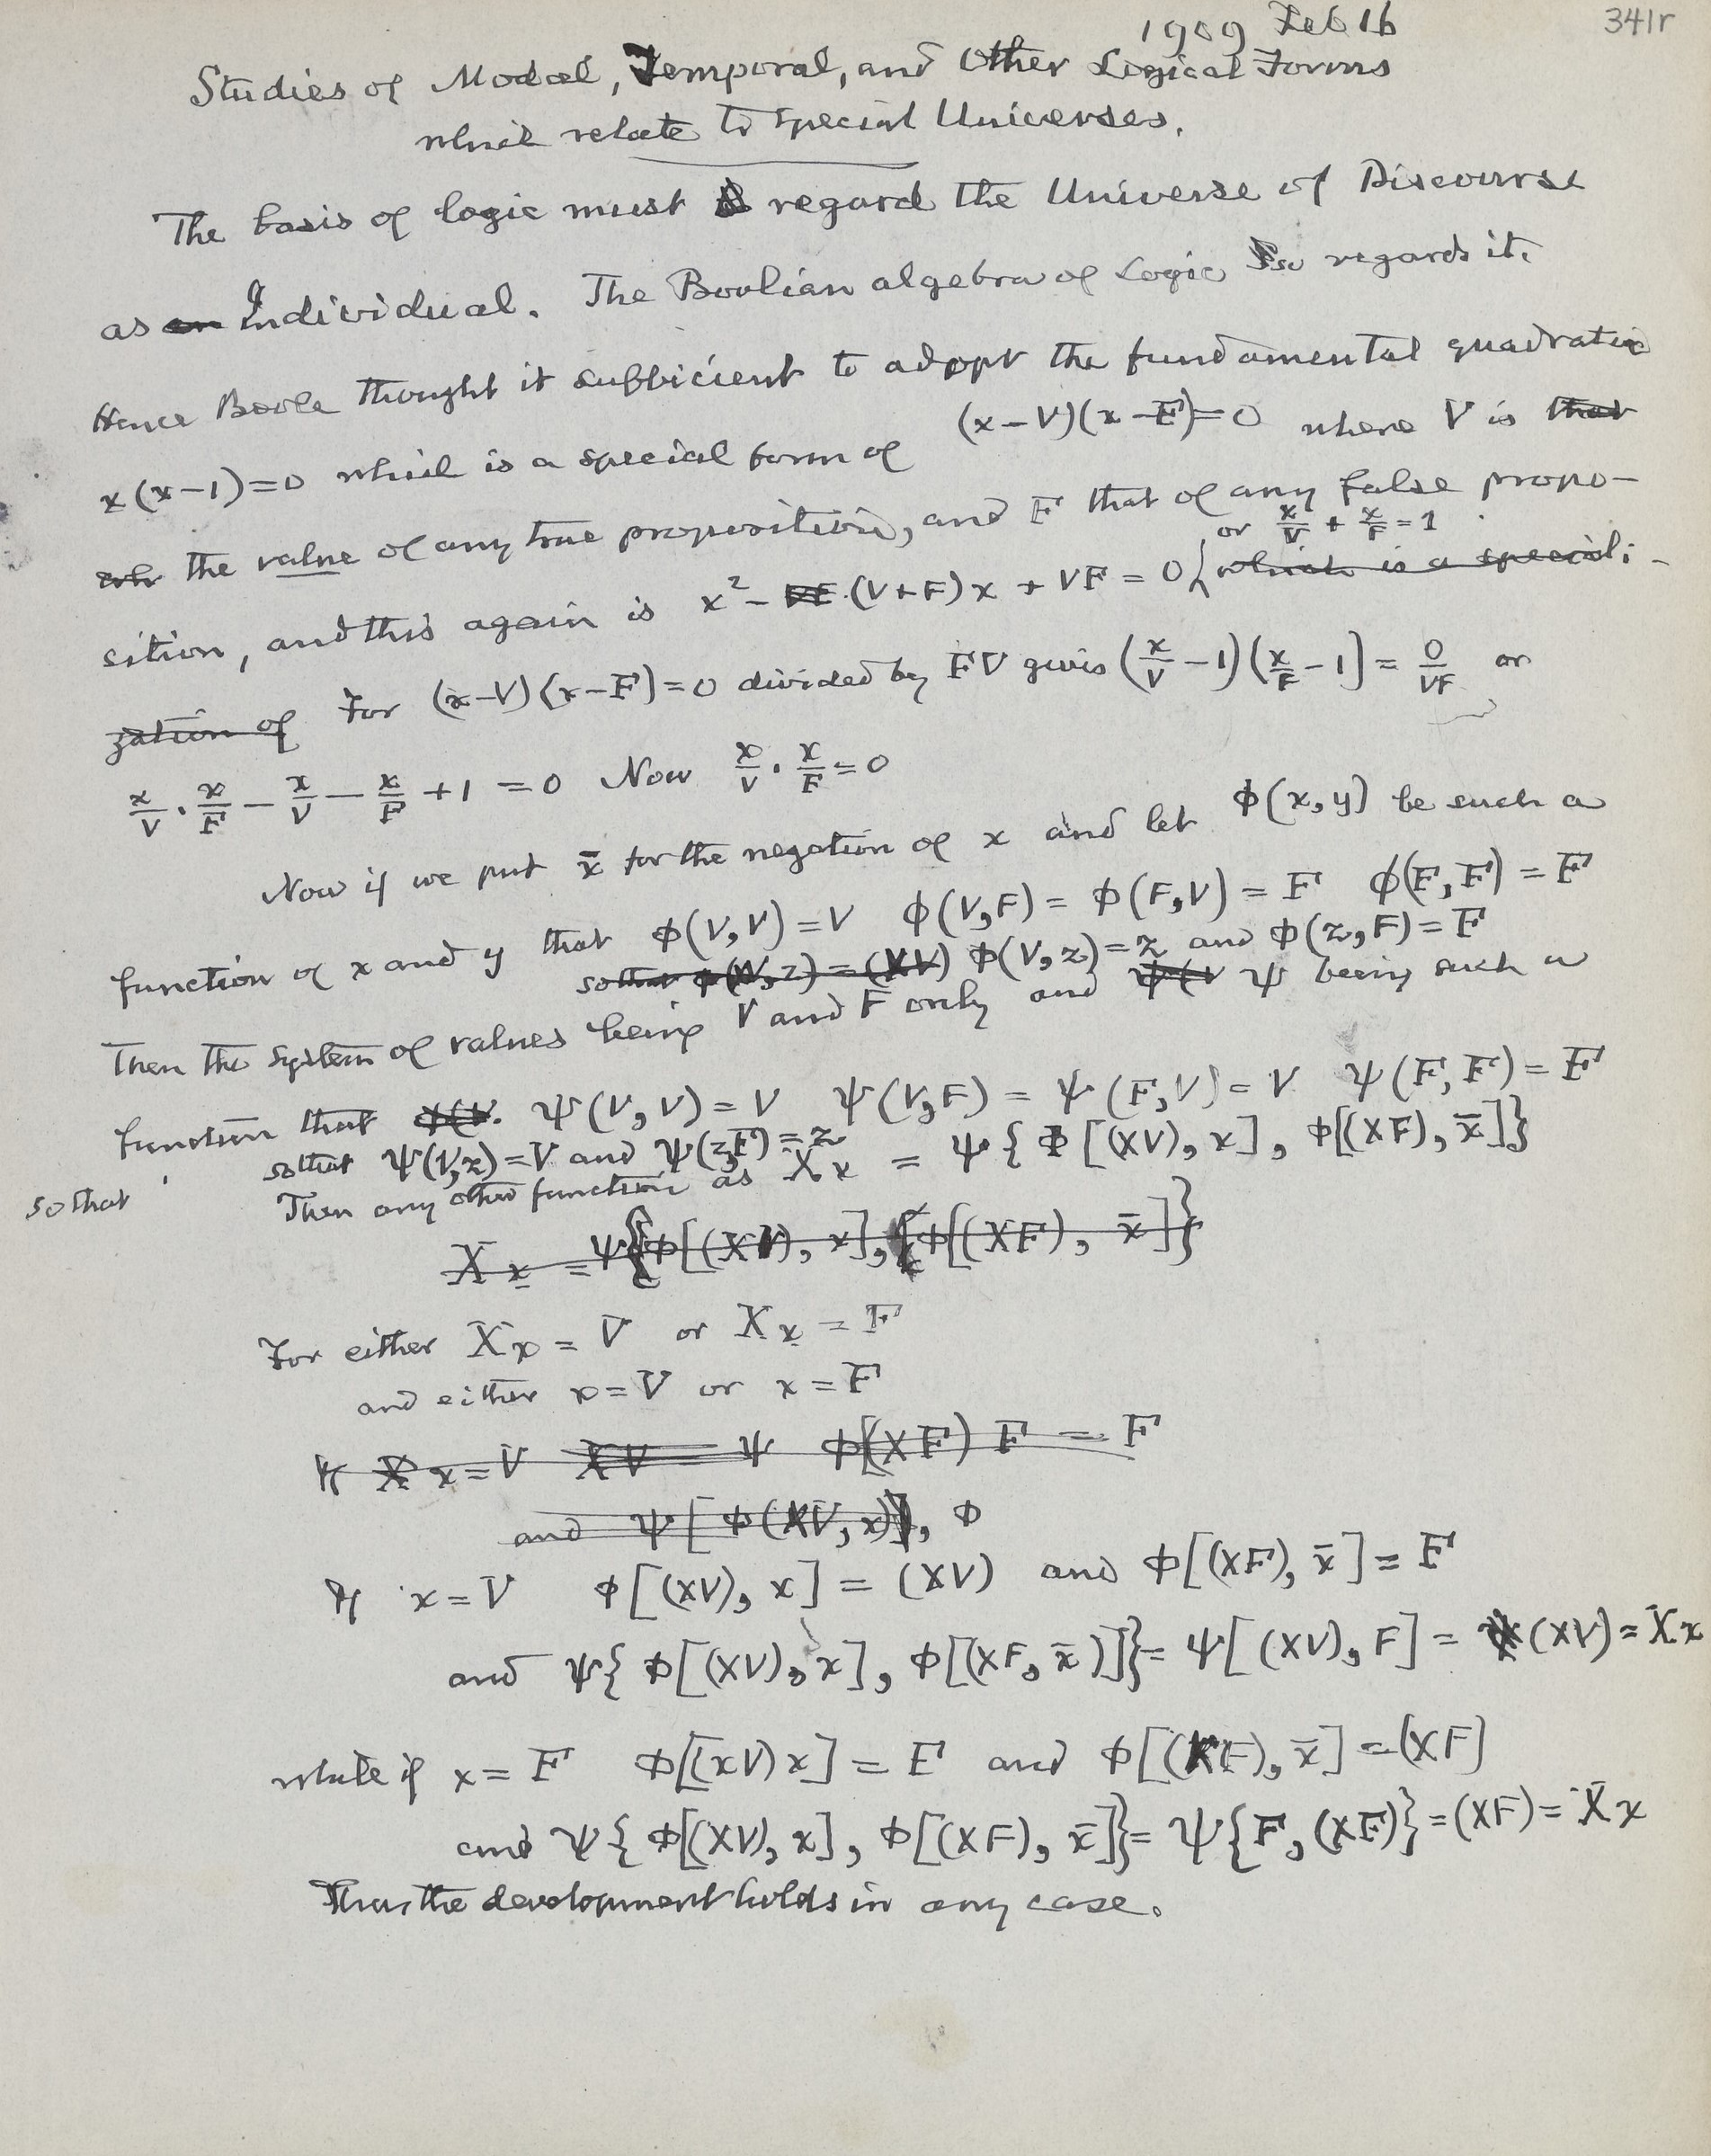
\includegraphics[width=\textwidth]{images/seq639.jpg}
    \caption{seq. 639 R.}
    \label{fig:639r}
\end{figure}

The next page up for discussion is the \textit{recto} that lies between the first two \textit{versos} that Fisch and Turquette discuss in their article. It is one of the few pages in Peirce's notebook that lends itself to a straightforward transcription. The page is dated February 16th, 1909 and its title reads as follows:

\begin{center}
\displayquote{``Studies of Modal, Temporal, and Other Logical Forms which relate to special Universes.''}
\end{center}

Here Peirce gives some further indication of the subject matter he is trying to capture, which appears to have something to do with temporal and modal propositions. It is unclear what the ``Other Logical Forms'' being referred to are, but one possibility is second order propositions since he had distinguished between first order and second order logic since at least 1885. But what does he mean by special universes? Elsewhere when Peirce speaks of special universes, it is in connection with his metaphysical categories and the ``modes of being'' discussed in section 3 of this chapter. In the same notebook, on August 28th in 1908, Peirce writes of ``the co-reality of three universes[:] 1st of ideas, 2nd of occurrences (existent things and actual events), [and] 3rd of powers to bring two substances $[\!\![$?$]\!\!]$, (and I will call powers of this sort Reasons), [which] must, accordingly, be supposed capable of rational explanation''(MS 339, \href{https://iiif.lib.harvard.edu/manifests/view/drs:15255301$550i}{seq.550}).\footnote{Fisch and Turquette draw attention to this passage as well.} This is most likely what Peirce was referring to when he writes ``special universes.'' Just as his `modes of being' are interpreted modally, so are his special universes. Peirce goes on to frame these special universes within his greater theory of ``hypothetical cosmology'' (\href{https://iiif.lib.harvard.edu/manifests/view/drs:15255301$555i}{seq. 555}).

The pages where Peirce elaborates this notion appears to be an outline of some kind. Based on the elaborations on the subsequent pages, we can infer that the `possibles' he is talking about do not necessarily only have the mode of being of possibility because they are unknown. They are not merely epistemically indeterminate. He calls them ``Real possibles.'' The `Reasons' he refers to are ``Real general Reasons, which do not merely exist in any mind of minds knowing that the denial of them are in no actual occurrence true.'' This is connected to something like what we might call `laws of nature.' For both of these concepts, Peirce is adamant in this passage that whatever they are is not `merely' epistemological. Their status as ``Possibles'' or ``Reasons'' is not based on our knowing whether they could pertain or our knowing that they could not not pertain. Peirce was an ardent defender of realism as opposed to nominalism, so this is likely the reason for this qualification.

The first paragraph on the page reads:
\begin{quotation}
\noindent``The basis of logic must regard the Universe of Discourse as individual. The Boolian algebra of Logic so regards it. Hence Boole thought it sufficient to adopt the fundamental quadratic $x(x-1)=0$ which is a special form of $(x-V)(x-F)=0$ where $V$ is the value of any true proposition, and $F$ that of any false proposition, and this again is $x^{2}-(V+F)x+VF=0$ (or $\frac{x}{V} +\frac{x}{F}=1$). For $(x-V)(x-F)=0$ divided by $FV$ gives $(\frac{x}{V} -1)(\frac{x}{F} -2)=\frac{0}{VF}$ or $\frac{x}{V} \cdot \frac{x}{F}-\frac{x}{V}-\frac{x}{F}+1=0$. Now $\frac{x}{V} \cdot \frac{x}{F}=0$''
\end{quotation}
\noindent The fundamental quadratic that Peirce refers too can be read as saying `it is false that some $x$ is not $x$' (as Boole used formulae of the form $x(1-y)$ to express `some $x$ is not $y$').\footnote{This is essentially a version of the Law of Identity.} The formula he says this is a special version of is a kind of ``elective expression,'' which in this case is simply the principle of non-contradiction (PC). Throughout this page he appears to be trying to extend this notion rather than refute it. Although, it is difficult to say what he was up to here because division does not seem to be part of Boole's notation, so it is unclear what he means when he writes expressions like $\frac{x}{V}$. One interpretation of the work on this page is that Peirce is attempting to modify an essentially Boolean system so that it can represent propositions involving the `special universes' he mentions in the title. If I am correct about the connection between these and the universes he described a few months prior, then he may have been trying to extend the scope of logic to propositions about possibilities and ``Reasons'', which might be understood as something like necessities.

Next $\Phi$ and $\Psi$ make an appearance again:
\begin{quotation}
``Now if we put $\bar{\lnot}x$ for the negation of $x$ and let $\Phi(x,y)$ be such a function that $\Phi(V,V)=V$, $\Phi(V,F)=\Phi(F,V)=F$, $\Phi(F,F)=F$. Then the system of values being $V$ and $F$ only and $\Psi$ being such a function that $\Psi(V, V)= V$ , $\Psi(V, F)=\Psi(F, V)=V$ , $\Psi(F, F)=F$

So that $\Psi(V, z)=V$ and $\Psi(x, F)= z$''
\end{quotation}
\noindent It may be worth noting that these formulations are inconsistent with the matrices written on the back of this page. Here it seems $\Phi$ and $\Psi$ have switched roles and now $\Phi$ is playing the role of conjunction and vice versa. In other regards they are consistent with the treatment of conjunction and disjunction in classical logic. He goes on to say:
\begin{quotation}
``Then any other function as $Xx=\Psi\{\Phi[(XV), x], \Phi[(XF),\bar{x}]\}$

For either $Xx=V$ or $Xx=F$

and either $x=V$ or $x=F$.''
\end{quotation}

\noindent This portion of the text helps to make sense of some of what appears on the first page Fisch and Turquette concern themselves with (seq. 639, \ref{fig:639r}). The portion of the page labelled (2) now appears to be making use of or working out a one place operator, $X$. So, when $XV$ appears within formulae in (4) and (5) of that same page, what is really meant is $X$ of $V$, $F$, or $x$. Here Peirce has given us a definition of that operator, however, the definition is clearly circular. This is likely no accident, and may have a connection with the third truth value, $L$, that appears on the other pages. Interpreting $\Phi$ as a kind of conjunction, and $\Psi$ as a kind of disjunction, we can see that $Xx$ will be reduced to either $XV$ or $XF$ depending on whether $x$ is true or not. If $x$ is true, then the right disjunct will be false, since $\bar{\lnot}x$ will be false, and the truth of the right disjunct will depend on the value assigned to $XV$. Likewise, if $x$ is false, then the value of $Xx$ will be whatever the value of $XF$ turns out to be. But of course we do not know what $XV$ or $XF$ will be because $X$ is used in its own definition. Peirce goes on to spell this out himself:
\begin{quotation}
``If $x=V$, $\Phi[(XV), x]=(XV)$ and $\Phi[(XF), \bar{x}]=F$

and $\Psi\{\Phi[(XV), x],\Phi[(XF), \bar{x}]\}=\Psi[(XV), F]= (XV)=Xx$

While if $x=F$, $\Phi[(XV), x]=F$ and $\Phi[(XF), \bar{x}]=(XF)$

and $\Psi\{\Phi[(XV), x],\Phi[(XF), \bar{x}]\}=\Psi\{(F, (XF)\}= (XV)=Xx$.''
\end{quotation}
The circular nature of the definition of $X$ might have some connection with the philosophical worries that led Peirce to begin these experiments in the first place. Perhaps it was introduced to represent portions of propositions whose truth value is either unknown or is fundamentally indeterminate. Peirce concludes this page stating ``Thus the development holds in any case.'' It is unclear what development Peirce is talking about but it likely has something to do with $X$. When he says it holds in any case, he may mean that it holds whether $x$ is true or false as in classical logic since maintaining this consistency seems to have been a priority.
%According to Richard he's showing that  X holds when the values are only T and F, and on the next page he is checking to see if it works for 3 values.

\section{seq. 641 R.}

\begin{figure}
    \centering
    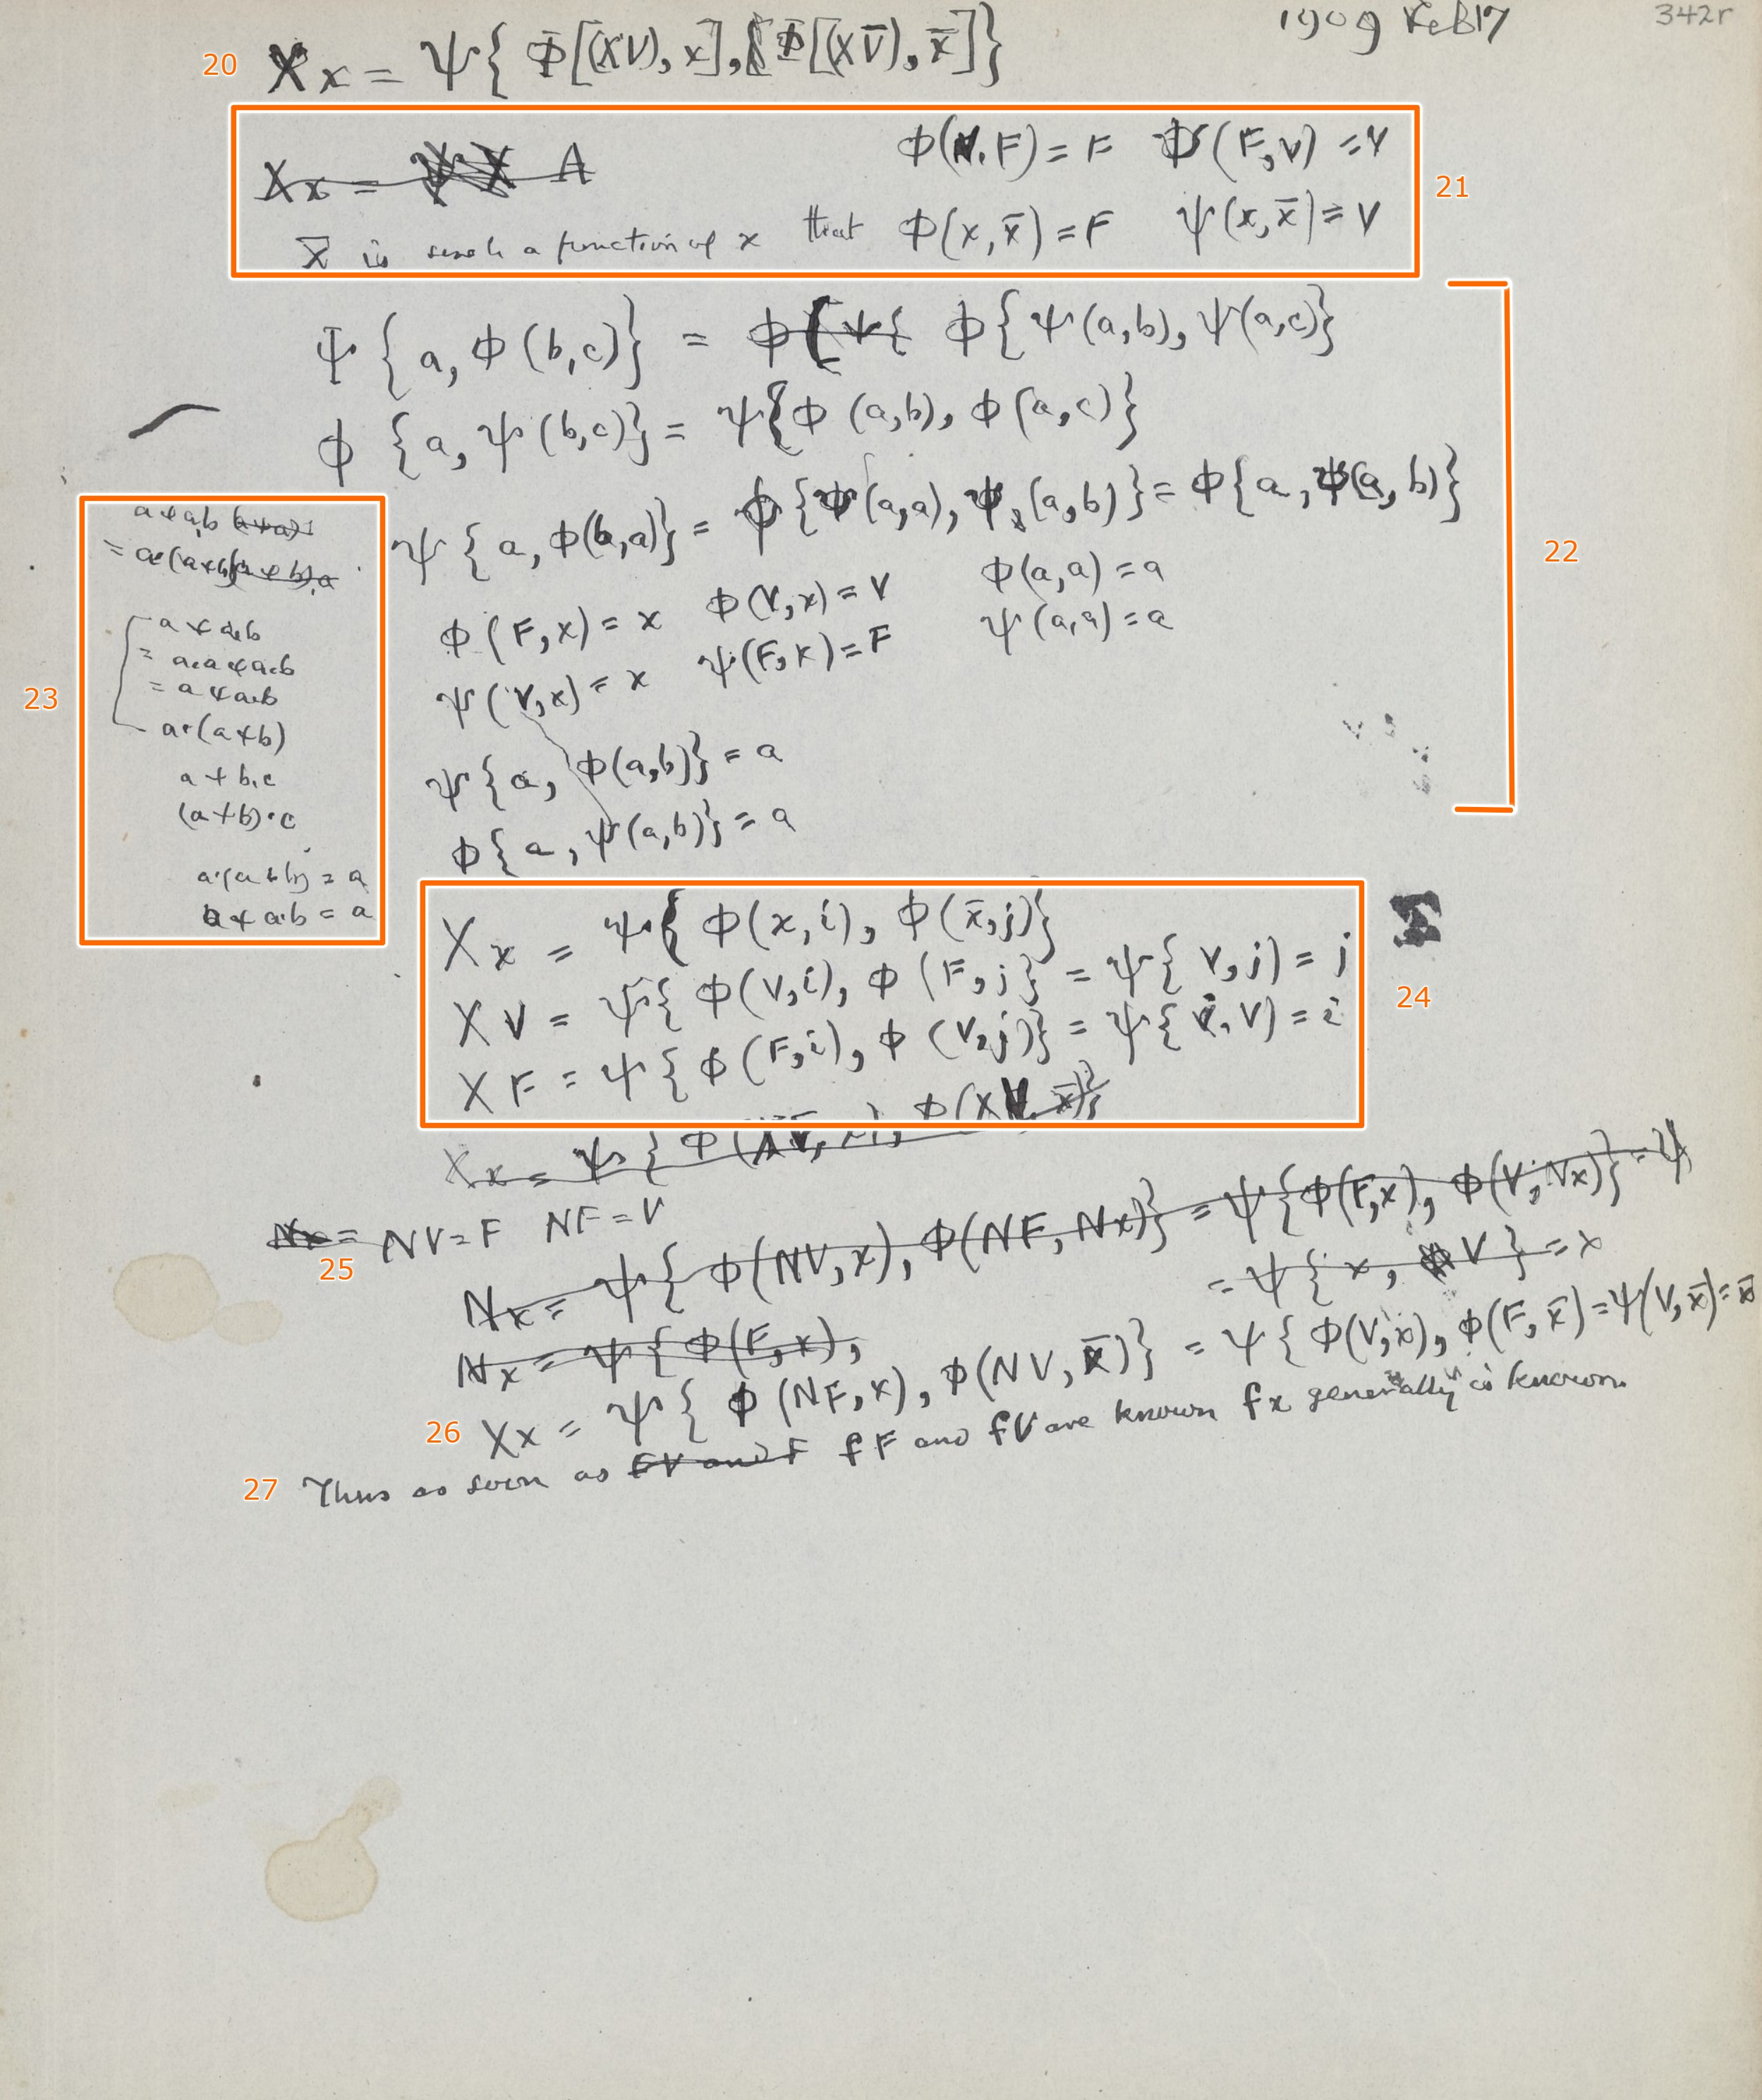
\includegraphics[width=\textwidth]{images/seq641.jpeg}
    \caption{seq. 641 R.}
    \label{fig:641}
\end{figure}

The final page in this group is a \textit{recto} following the second page Fisch and Turquette take up. It is dated February 17th, 1909.

The page begins (20) by recapitulating the definition for $X$. The only difference between the definition here and that of the previously discussed page is that instead of $F$ Peirce writes $V$ with a line above to symbolize its negation: ``$Xx=\Psi\{\Phi[(XV), x], \Phi[(X\bar{V}),\bar{x}]\}$''. This doesn't seem to amount to a significant change.

In (22) he restates some features of $\Phi$ and $\Psi$ as well as the negation operator, $\bar{\lnot}x$ (which is presumably the three-valued version). It reads ``$\Phi(V,F)=F$, $\Psi(F,V)=V$'' and then states that ``$\bar{\lnot}x$ is such a function that $\Phi(x,\bar{x})=F$ [and] $\Psi(x, \bar{x})=V$.'' So again, $\Phi$ and $\Psi$ are working like regular conjunction and disjunction. It also seems as though he is trying to show that the laws of non-contradiction and excluded middle still hold with regard to $\bar{\lnot}x$. 

Immediately below (22), he gives some basic equivalences between $\Phi$ and $\Psi$ formulae before giving formulations that contradict what is written of $\Phi$ and $\Psi$ in (21) and seq. 639. It seems that either here or while scribbling on the \textit{verso} facing this page Peirce had decided to switch the roles of $\Phi$ and $\Psi$. $\Phi$ is now a kind of disjunction and $\Psi$ now a kind of disjunction. There is no apparent reason for doing this, so it likely came down to personal preference.

To the left (23), there appears to be some scratch work that contains formulae misshapen $+$ signs, which could be $\Psi$s but are more likely regular two valued disjunctions. They appear alongside $\cdot$s, which are normally two valued conjunctions in Peirce's notation. The connectives are combining arbitrary atomic sentences, but it is unclear what the overall significance of this is.

In (24), we find more formulations with $X$. He writes:
\begin{quotation}
``$\Psi\{\Phi(x, i),\Phi(\bar{x}, j)\}$

$\Psi\{\Phi(V, i),\Phi(F, j)\}=\Psi(V,j)=j$

$\Psi\{\Phi(F, i),\Phi(V, j)\}=\Psi(i,V)=i$''
\end{quotation}
\noindent One difference between these formulations and his previous characterization of $X$ is that $\Psi$ and $\Phi$ roles have switched, which is consistent with (22), yet $\Psi$ is still the primary operator in the definitions. Another difference is that the circularity of the previous definition has been dropped. $X$ no longer features in its own definition. The final difference is that $i$ and $j$ have been added to the mix aside from $x$, $V$, and $F$. He may have had specific interpretations in mind for these, but the only other place they show up in these pages is in \href{https://iiif.lib.harvard.edu/manifests/view/drs:15255301$637i}{seq. 637}, where they are winners and losers. It is doubtful that this is what they mean here though.

The next line (25) introduces something new. Here Peirce has written ``$NF=F$ [and] $NF=V$.'' He tells us very little about this new operator but it may be of a similar kind to $X$. One possibility is that these were intended to be kinds of modal operators, as he seems to have been concerned with modality on previous pages. It is unclear whether either of them are intended to be truth-functional. Nevertheless, $N$ appears in connection with $X$ in the next line (26): ``$Xx=\Psi\{\Phi(NF, x), \Phi(NV, \bar{x})\}=\Psi\{\Phi(V,x),\Phi(F,\bar{x}\}=\Psi(V,\bar{x})=\bar{x} $.'' This formula is basically the same as the definition for $X$ on the previously discussed page except the $X$s on the right of the identity symbol are replaced with $N$s. But since we know that $NF=F$ and $NF=V$, the value of the formula is able to be reduced to the value of $\bar{\lnot}x$. 

The most interesting part of the page is likely the last line(27). In it Peirce states ``Thus as as soon as $fF$ and $fV$ are known $fx$ is generally known.'' The $f$ here seems most likely to be an arbitrary place holder for unary functions like $X$ and $N$. It is unclear how best to interpret this. It is possible that Peirce may simply be claiming that if you know what a function on \textit{Verum} and \textit{Falsum} give you, then figuring out what that function gives on any arbitrary proposition is a trivial matter.


\chapter{Philosophical motivations}

It took decades before Peirce's generalization of the matrix method to three values was even discovered. The first mention of this development seems to have been in an article Turquette produced for an edited volume entitled \textit{Studies in the Philosophy of Charles Sanders Peirce} \citep{turquette1964studies}. To date, the only attempts there seem to have been to exposit Peirce's philosophical motivations are due to Fisch and Turquette \citeyearpar{fisch_peirces_1966}, and Lane \citeyearpar{lane_peirces_1999}. After Fisch and Turquette published that first article together, Turquette went on to develop various formal aspects of Peirce's triadic logic, mostly ignoring the philosophical side of the equation.

In this section, I will give an account of each of these attempts to explain why Peirce saw the need to deviate from the classical two valued logic he helped to create, and weigh their claims against the evidence that can be gleaned from Peirce's notebook. Fisch and Turquette lean towards his notions of triadic modality as an explanation, however they offer a couple of other possibilities along the way. Lane on the other hand, insists that modality had nothing to do with the matter, and instead draws his explanation based on Peirce's views on continuity and continua. I will first give an account of Fisch and Turquette's views and then turn to Lane.

\section{Max Fisch and Atwell Turquette's account}

Fisch and Turquette begin by discussing the various operators and formal developments on the first three pages of the notebook I have discussed. They note that on the formal side, Peirce seems to have been motivated by a concern for duality and functional completeness when he defined his operators as demonstrated by the fact that every one of them has its $\bar{x}$ dual defined also. But when it comes to his philosophical reasons, Fisch and Turquette are much more tentative. They offer roughly three possibilities: 1) that Peirce was motivated by considerations of modality, as Łukasiewicz was, 2) that his motivations were due to his doctrine of ``Tychism,'' which basically holds that there is fundamental indeterminacy in the world, and 3) that his triadic logic was connected to the ``three dimensional logic'' of Hugh MacColl, who was a long time correspondent of Peirce.

They begin their explanation stating that ``It is clearly indicated that the motivation arises from problems associated with the kind of proposition which `has a lower mode of being such that it can neither be determinately $P$, nor determinately not-$P$' --- assuming that the proposition in question is of the form $S$ is $P$'' \citep[77]{fisch_peirces_1966}. They draw this evidence from \href{https://iiif.lib.harvard.edu/manifests/view/drs:15255301$645i}{seq. 645}, where Peirce states as much himself, and claim that this is enough to suggest that he was motivated by concerns for modality, as Łukasiewicz was. More specifically, they claim he was interested in modal issues in which a third truth value seems necessary to evaluate propositions, such as future contingents. The most famous example is Aristotle's future sea battle case. If I pronounce `there will be a sea battle tomorrow', at the time of my utterance it is unclear what the truth value of the proposition is. Whether or not there does happen to be a sea battle the next day, it may still seem inappropriate to say the proposition is true or false, and we may want to reserve an intermediate value for the proposition. Nonetheless, Peirce's one remark on \href{https://iiif.lib.harvard.edu/manifests/view/drs:15255301$645i}{seq. 645} seems rather thin evidence to justify the claim that it was these kinds of modal propositions he was hoping to capture.

To further support their claim, Fisch and Turquette draw our attention an entry in \textit{The Prescott Book} (MS 277) from January 1908. The passage discusses modality in connection with ``potentiality'', ``actuality'', and ``necessitation'' \citep{fisch_peirces_1966}. It reads: \begin{quotation}
\noindent\textit{Potentiality} is the absence of Determination (in the usual broad sense) not of a mere negative kind but a positive capacity to be Yea or Nay; not ignorance but a state of being...\\ \textit{Actuality} is the Act which determines the merely possible...\\ \textit{Necessitation} is the support of Actuality by reason...
\end{quotation}
\noindent They then go on to cite the passage concerning the three universes in the Logic Notebook from August 1908 (\href{https://iiif.lib.harvard.edu/manifests/view/drs:15255301$550i}{seq. 550}). This provides evidence that Peirce was thinking about modality throughout the year leading up to his experiments in triadic logic. It also provides a possible explanation of what Peirce meant when he writes of lower modes of being on \href{https://iiif.lib.harvard.edu/manifests/view/drs:15255301$645i}{seq. 645} (\ref{fig:645}). His comment seems to imply a commitment to a hierarchy of modes of being, and it certainly makes sense to think of ``potentiality'' being at the bottom and ``necessitation'' on the top if he really was concerned with modality. Furthermore, if I am correct that there is a connection between the ``special universes'' in the title of \href{https://iiif.lib.harvard.edu/manifests/view/drs:15255301$639i}{seq. 639} (\ref{fig:639r}) and the ``three universes'' Peirce discusses in the notebook previously, then this would be strong evidence in favor of Fisch and Turquette's view that he was operating with some notion of modality in mind.

Peirce continued thinking and writing about modality in triadic terms throughout the final years of his life and it seems fairly clear that when he did so he had this kind of hierarchy in mind. In an unpublished essay cited by Fisch and Turquette, entitled \textit{The Art of Reasoning Elucidated}, he writes:\begin{quotation} \noindent``Now, in this respect, a simply assertory proposition differs just half as much from the assertion of a Possibility, or that of a Necessity, as these two differ from each other. For, as we have seen above, that which characterizes and defines an assertion of Possibility is its emancipation from the Principle of Contradiction, while it remains subject to the Principle of Excluded Third; while that which characterizes and defines an assertion of Necessity is that it remains subject to the Principle of Contradiction, but throws off the yoke of the Principle of Excluded Third; and what characterizes and defines an assertion of Actuality, or simple Existence, is that it acknowledges allegiance to both formulae, and is thus just midway between the two rational ``Modals'', as the modified forms are called by all the old logicians.'' (MS 678, 1910)\end{quotation}
\noindent Notice that when Peirce writes of ``Actuality'' he locates it between the possible and the necessary, suggesting a hierarchical ordering. Some of what is contained in this passage is perfectly consistent with the way we currently think of modal propositions too. While we would not normally say that the law of non-contradiction does not apply to modals, it is trivial to say that for any possible proposition $P$, `it is possible that $P$ and it is possible that not $P$.' This is likely what Peirce means when he claims potentials are emancipated from this principle. We can say something similar with regard to necessities and the principle of excluded middle. While we would not say that PEM fails for necessary statements, we also would not say of any proposition $P$ that `it is necessary that $P$ or it is necessary that not $P$' since it could be the case that neither. This is likely what Peirce meant when discussing these principles, although admittedly, this is not the standard way of understanding either of them.

Fisch and Turquette also use these notions to clarify what Peirce says on \href{https://iiif.lib.harvard.edu/manifests/view/drs:15255301$645i}{seq. 645} (\ref{fig:645}). They claim ``Essentially, Peirce seems to be saying that triadic logic may be interpreted as a modal logic which is designed to deal with the indeterminacies resulting from that mode of being which Peirce has called `Potentiality' and `Real Possibility''' \citep{fisch_peirces_1966}. This is why on that page Peirce claims that dyadic logic is ``not universally false it is only $L$.'' He may be saying that dyadic logic is limited because it fails to account for these real indeterminacies.

This brings us to their second point about Peirce's possible motivations: his Tychism. Unlike other philosophers working on logic around the time these pages were written, Peirce was committed to the view that there is fundamental indeterminacy in the world that cannot be removed by rendering propositions less ambiguous.\footnote{Unlike Bertrand Russell who in 1906 seems to have held that indeterminacy can always be removed by carrying a propositions determination further. So, for example, the indeterminacy of the proposition `Mrs. Brown is at home' can be removed by making the proposition more specific, i.e. by specifying a time and date, as in `Mrs. Brown was at home on the afternoon of \today.' \citep{russell_review_1906}} For Peirce, this indeterminacy is metaphysical in nature, and does not necessarily result merely from a lack of knowledge or the language we use. This follows from his 1898 definition of Tychism, as ``the doctrine that absolute chance is a factor in the universe'' (CP 6.201). Contrary to some authors of his time, like Russell, Peirce did not believe that ``the universe is [necessarily] regulated by law down to every detail" (Ibid). He was not a determinist, and thought that some facts of the world might come down to arbitrary chance. A little less than two weeks after he completed \href{https://iiif.lib.harvard.edu/manifests/view/drs:15255301$645i}{seq. 645} (\ref{fig:645}), Peirce writes in a letter to William James ``I hold to my `tychism' more than ever.' Fisch and Turquette use this evidence to connect Peirce to others who have held a similar belief in some kind of irreducible indeterminacy, like Hans Reichenbach or Werner Heisenberg, both of whom were motivated by undecidable statements about quantum mechanics. They further remark that Gödel's undecidable statements in mathematics could be another example of this kind of indeterminacy. Obviously Peirce could not have been aware of any of these developments, however his tychism might be seen as anticipating these kinds of results.

So it seems that Peirce's introduction of the value `$L$' to logic may have been a way of importing his tychism to logic. This would be consistent with complaints Peirce made about the ``oldfashioned logicians''\footnote{Presumably, these are more conservative logicians who were resistant to the advances made in logic by Boole, De Morgan, and Peirce, in favor of traditional syllogistic logic.} in a draft of the just mentioned letter, written just three days after seq. 645 (\ref{fig:645}). According to Fisch and Turquette's reproduction, it reads:
\begin{quotation} 
\noindent``I have long felt that it is a serious defect in existing logic that it takes no heed of the \textit{limit} between two realms. I do not say that the Principle of Excluded Middle is downright \textit{false}; but I \textit{do} say that in every field of thought whatsoever there is an intermediate ground between \textit{positive assertion} and \textit{positive negation} which is just as Real as they. Mathematicians always recognize this, and seek for that limit as the presumable lair of powerful concepts; while metaphysicians and oldfashioned logicians, --- the sheep [and] goat seperators, --- never recognize this. The recognition does not involve any denial of existing logic, but it involves a great addition to it.''
\end{quotation}
\noindent Is Peirce making reference to his triadic logic here? His remarks about this ``Real intermediate ground'' may be driven by his commitment to his tychism. Furthermore, his remarks here that acknowledging such a middle ground ``does not involve any denial of existing logic, but it involves a great addition to it'' seem awfully similar to his remarks about the difference between dyadic and triadic logic on \href{https://iiif.lib.harvard.edu/manifests/view/drs:15255301$645i}{seq. 645} (\ref{fig:645}). Thus, it seems Peirce's three-valued efforts might be an attempt to insert his tychism into logic. This explanation of Peirce's motivation is not necessarily distinct from the possibility that he was motivated by modal considerations, but it may help elucidate his understanding of modality.

The final point that Fisch and Turquette investigate has to do with the extent to which Peirce's triadic logic was related to the ``three dimensional'' logic of his long time correspondent, Hugh MacColl. MacColl's approach to logic involves a division of statements into three kinds: certain, impossible, and variable \citep{maccoll_symbolic_1906}. His logic is to a certain extent three-valued in that it accounts for the kinds of propositions he calls ``variable,'' which he sometimes refers to as `possible.' However, it is unclear whether he intended these variable propositions to take on a intermediate truth value, or if they were of unknown value and his logic contained truth gaps. This difficulty has led some to claim that MacColl is not actually a pioneering figure in the many-valued turn in logic \citep{conjunction_peter_1998}. However, it could be argued that any logic that admits truth gaps might just as easily be interpreted as a three-valued system, where the gaps are interpreted as the additional value.

Questions of his status in the history of non-classical logic aside, there is strong evidence that Peirce was aware of this particular aspect of MacColl's work. The two had been long time correspondents and admirers of each others work. In 1906, Peirce wrote a draft of a letter to MacColl inquiring about his new book:
\begin{quotation}
``P.O. Millford Pa 1906 Nov 16

My dear Sir:

Although my studies in symbolic logic have differed from yours in that my own aim has not been to apply the system to the working out of problems, as yours has, but to aid in the study of logic itself, nevertheless I have always thought that you alone, so far as I know, except myself, have understood how the matter ought to be treated by making the elements propositions on predicates and not common nouns. I beg have to send you here with a paper setting forth, in outline only, my system of existential graphs, which exhibits the logic of relations in the simplest possible manner.

I see by ``Nature'' of Nov 1 that you have a new book on the subject. My circumstances are so reduced that I can no longer purchase books. I notice them, however, for three or four important journals in this country, and should like very much to hear...'' (L 261).\footnote{Letter 261 in \textit{The Robin Catalogue}.}
\end{quotation}
\noindent The draft does not appear to ever have been completed and it is unclear whether he wrote to MacColl this late in his life. However, the draft does indicate that Peirce was aware of MacColl's later work. The article in ``Nature'' that he refers to here is a book review covering four volumes on logic released that year, among them MacColl's \textit{Symbolic Logic and its applications}. It makes explicit reference to MacColl's inclusion of variable propositions and notes a couple of criticisms against the feature. Thus, it is also likely that Peirce was aware of the aspect of MacColl's logic that bears a connection to his own triadic logic. Perhaps the reason for Peirce's interest in MacColl's book was that he thought it might offer some help with the issues concerning triadic modality that so consumed him around this time. However, Peirce never explicitly mentions MacColl or his book elsewhere so it is unlikely the connection goes any further than this.

Fisch and Turquette seem to make a strong case that in experimenting with three-valued logic, Peirce was motivated by concerns for his doctrine of tychism, which more broadly factors into his understanding of modality. At this point it seems likely that Peirce, like Łukasiewicz, thought it necessary to deviate from classical logic in order to deal with certain kinds of modal propositions. This connection is strengthened by considering some of what is written on the pages Fisch and Turquette neglect to mention. However, this suggestion runs contrary to the view Lane takes on Peirce's experiments. There is one major defect with Fisch and Turquette's account and this is that they pay no special attention to Peirce's ink blot example on \href{https://iiif.lib.harvard.edu/manifests/view/drs:15255301$645i}{seq. 645} (\ref{fig:645}). The only mention of it is in a sentence that declares it ``is not very helpful in providing an answer'' \citep{fisch_peirces_1966}. Lane's account explores this example in much greater detail.

\section{Robert Lane's account}

Writing more than 30 years after Fisch and Turquette, Robert Lane expresses an explicitly very different view of what Peirce was up to with his triadic logic. On Lane's view, Peirce was motivated not by concern for modality, but by his understanding of continuity and the continuum. In this section I will elaborate on Lane's account of Peirce's motivations. I will begin by explaining why Lane thinks we should reject the view that locates Peirce's motivation in the realm of modality. I will then elaborate on Lane's positive claim, that Peirce was instead motivated by issues resulting from continuity.

Lane's route to his denial that Peirce was not here concerned with triadic modality is somewhat long. It begins with an exposition of Peirce's views on the principle of excluded middle (PEM) on the one hand, and the principle of non-contradiction (PC) on the other. His account here is an expansion of a previous paper on PEM and PC \citep{lane_peirces_1999}.

A crucial distinction involved with Peirce's understanding of these principles, according to Lane, ``is the distinction between saying of a logical principle, on the one hand, \textit{that it does not apply to a proposition}, and on the other, \textit{that it is false with regard to that proposition}" \citep{lane_peirces_1999}. According to this distinction, Lane claims that Peirce's $L$-propositions are ones that PEM still \textit{applies} to, but is nonetheless false in regards to. There are some obvious difficulties with this distinction, and it may involve a less than standard view of what it is to be a logical principle. It is not at all clear what sense there is in saying that a logical principle applies to a proposition that falsifies it. At face value, it seems a proposition that makes PEM false is precisely a proposition that PEM does not apply to. Lane indicates that Peirce made this distinction only once in a manuscript written in the same year he created his triadic logic, but he does not indicate exactly where this page can be found. Nevertheless, these remarks are somewhat consistent with Peirce's claim on \href{https://iiif.lib.harvard.edu/manifests/view/drs:15255301$645i}{seq. 645} (\ref{fig:645}) that triadic logic ``does not reject entirely the principle of excluded middle.''

While Peirce may have only made this particular distinction once, there are plenty of examples of him writing about propositions that PEM and PC do not apply to (though he doesn't say they are false in regard to these propositions). These are always general propositions and vague propositions respectively. As an example of this, Lane draws our attention to the following passage: ``anything is \textit{general} insofar as the principle of excluded middle does not apply to it and is \textit{vague} insofar as the principle of contradiction does not apply to it. '' (CP 5.448, \textit{Issues in Pragmaticism}, 1905). Notice the similarity between Peirce's remark here and his remarks about potentials and necessities in connection with PEM and PC discussed in the previous section. According to Lane, by general propositions Peirce really meant universally quantified propositions. The evidence for this is Peirce's use of the proposition ``Man is mortal'' as an example of a general proposition \citep{lane_peirces_1999}. However, that proposition might be importantly different from the proposition ``All men are mortal.'' In the original proposition, Lane rightly claims that ``Man'' is being used as a ``general propositional subject.'' But this might be because the word ``man'' is a general sign and we would require an exposition of Peirce's semiotic theory to hash out whether this means the same thing as ``All men'', which is more clearly a quantificational subject.

This aside, the reason Peirce gives for why PEM does not apply to general propositions is that ``the general is partially indeterminate.'' In the passage Lane draws this example from, Peirce gives a somewhat different definition of what a general proposition is: ``A sign\dots, that is in any respect objectively indeterminate (i.e., whose object is undetermined by the sign itself) is objectively \textit{general} in so far as it extends to the interpreter the privilege of carrying its determination further. Example: `Man is mortal.' to the question, What man? the reply is that the proposition explicitly leaves it to you to apply its assertion to what man or men you will.'' (CP 5.447) There is a footnote in this passage in which Peirce does mention universal propositions only to note that they are distributively general rather than collectively general. The significance of this is unclear but it does seem to connect generals to universals. Although, the definition he gives in the above passage makes no mention of ``universally quantified propositions.'' 

While there may be difficulties with interpreting generals straightforwardly as universally quantified propositions, Lane takes this and Peirce's statement about PEM to imply that Peirce had a non-standard view of PEM. He introduces two modes in which Peirce may have understood PEM: a material mode and a formal mode.\footnote{This distinction is due to Carnap.} According to the material mode, PEM States: ``for any property and for any individual, either that individual possesses that property or that individual does not possess that property.'' In the formal mode: ``for any pair of contradictory predicates `$P$' and `not-$P$' and for any individual (non-general) subject-term `$S$', either `$S$ is $P$' or `$S$ is not-$P$' is true. (The evidence that Peirce might have thought of PEM this way comes from MS 611 and CP 1.434.) So, on Peirce's understanding, PEM applies only to individual subjects, not generals like properties or predicates.\footnote{So, put simply, where we would normally interpret PEM with respect to general propositions as stating `$\forall x P(x) \lor \neg \forall x P(x)$,' Peirce would have interpreted it as stating `$\forall x P(x) \lor \forall x \neg P(x)$' which is clearly very different.} According to Lane, this is why Peirce claims PEM is sometimes false with regard to general propositions. When the subject of a proposition is general rather than individual, PEM can fail, as in Lane's example ``All Floridians are Miamians or All Floridians are non-Miamians" \citep{lane_peirces_1999}.

Peirce seems to have understood PC in essentially the same way and Lane goes on to spell out the material and formal modes for it as well. What this all amounts to is basically that Peirce's claim that PEM does not apply to generals in conjunction with his idiosyncratic understanding of the principle does not pose a threat to our standard way of thinking about PEM.

Because of his non-standard way of understanding PEM and PC, Lane claims Peirce's denial of PEM applying to generals (or necessities) and of PC applying to vague propositions (or potentials) does not involve any denial of bivalence. This is true since if PEM and PC are restricted to individuals, this does not mean that propositions about these individuals are anything other than true or false. Peirce also claims that PEM and PC not apply necessary and possible propositions for the same reasons they do not apply to generals and vague propositions. Lane takes this lack of conflict with bivalence to demonstrate that Peirce's triadic logic had nothing to do with modality. The argument can be restated as follows: 
\begin{enumerate}
\item Triadic logic must involve a rejection of bivalence. 
\item The denial of PEM applying to necessary propositions and PC applying to possible propositions does not involve a rejection of bivalence.
\item So, Triadic logic could not have been motivated by modality.
\end{enumerate}
While Peirce does not explicitly mention PB anywhere on the pages about triadic logic, it must have been rejected, since any logic that admits a third truth value inherently denies bivalence. Nonetheless, this argument is not valid. The reason for this is that, while Peirce's rather odd understanding of PEM and PC do not require a resection of bivalence it also does not necessitate its acceptance. So, even though Peirce's understanding of modality, does not require rejecting bivalence, this alone is not enough to justify the claim that modality had nothing to do with it.

Aside from the invalidity of this argument, if we were to accept it this would create some explanatory gaps in our account. How would we explain Peirce's use of the phrase ``modes of being'' which he almost certainly understood in modal terms at the time of writing? Furthermore, why would he have put modality in the title of \href{https://iiif.lib.harvard.edu/manifests/view/drs:15255301$639i}{seq. 639} (\ref{fig:639r}) if modality had nothing to do with his project? For these reasons I think we think we should reject Lane's negative point and continue to entertain the possibility that modality was a motivating factor for triadic logic. Lane goes on to argue further that when Peirce was conducting his triadic experiments that he was concerned with propositions of which PEM applies, but is nonetheless false with regard to, returning to the distinction he made earlier. But this would seem to fly in the face of Peirce's claim on \href{https://iiif.lib.harvard.edu/manifests/view/drs:15255301$645i}{seq. 645} (\ref{fig:645}) that PEM is ``not necessarily false'' in regard to triadic logic. It seems more likely that he would say PEM is not false about those propositions, but that it is merely `$L$'.

 The issues with Lane's negative claim by no means undermine the value of his positive claim: that Peirce was motivated by issues surrounding continuity. Continuity was a major concern in Peirce's philosophy throughout the entirety of his life, and especially in this later period. He came to it not only through his own philosophical lens, but also from reading other influential figures, like Cantor,  Dedekind, and Bolzano (more on this in the next chapter). Lane comes to this contribution by exploring an aspect of seq. 645 (\ref{fig:645}) that Fisch and Turquette almost entirely neglect: his inkblot example.
 
 The inkblot example is the only explicit reference to the kinds of propositions the value $L$ is supposed to be assigned to. The example restated reads: 
\begin{quotation}
\noindent``Thus, a blot is made on a sheet. Then every point of the sheet is unblackened or blackened. But there are points on the boundary line; and those points are insusceptible of being blackened or of being unblackened, since these predicates refer to the area about $S$\footnote{$S$ here is the subject of the proposition, the boundary line.} and a line has no area about any point of it.''
\end{quotation}
\noindent At face value, Peirce's example appears to be concerned with cases of predication involving category mistakes, however Lane's analysis reveals that it is more likely about breaches of continuity. Lane claims that the individual subject being Considered here is the boundary line, $B$. The proposition `$B$ is black' then would relieve the valuation $L$ because it is not true that $B$ is black, nor that $B$ is not. Rather, Lane claims quoting Peirce, $B$ ``is at the limit between [black] and non-black]" (Lane, 1999). $B$ in this example, constitutes a breach of continuity. It interrupts at the continuous space on the sheet of paper, and lacks the properties possessed by the regions on either side. Given the importance Peirce placed on continuity elsewhere in his philosophy, this is a much more natural interpretation of the example than category mistakes (although calling $B$ black is, in a sense, still a kind of category mistake on this view).
 
 It might seem odd that Peirce would place so much importance on such a narrow range of propositions that he thought it necessary to revise logic to accommodate them. But Peirce thought continuity was of the utmost importance, and so breaks in continuity would also have been important to him. To illustrate this importance, Lane draws our attention to this passage:
 \begin{quotation}
\noindent``[T]he idea of continuity, or unbrokenness\dots plays a great part in all scientific thought, and the greater the more scientific that thought is; and it is the master key which adepts tell us unlocks the arcana of philosophy'' (CP 1.163).
\end{quotation}
\noindent Peirce's emphasis on continuity in philosophy and in science stems from another doctrine that he endorsed, not altogether unlike the previously mentioned doctrine of tychism. He called this synechism, and says it is the ``doctrine that all that exists is continuous'' (CP 1.172). His reasons for endorsing synechism are far beyond the scope of this thesis, but he likely perceived the continuity of time, space, and thought as evidence supporting his endorsement.

There is further textual evidence to support the link between the inkblot example and Peirce's views on continuity. He used a similar example in the eighth of his Cambridge Conference lectures in 1898 (CCL, all of which are presented in \cite{peirce_reasoning_1992}), which Lane quotes from, where he is quite clearly talking about continuity and boundary properties:
\begin{quotation}
\noindent``I draw a chalk line on the board\dots what I have really drawn there is an oval line. For this white chalk-mark is not a line, it is a plane figure in Euclid’s sense---a surface, and the only line there is the line which forms the limit between the black surface and the white surface\dots the boundary between the black and white is neither black; nor white, nor neither, nor both.'' (CP. 6.203)\label{laneq}\footnote{I present this passage here as Lane does in his paper. We will soon see, briefly in this chapter and extensively in the final chapter, there are a lot of relevant details in the ellipses.}
\end{quotation}
\noindent The inkblot example seems pretty clearly to be a brief expression of the ideas Peirce was elaborating here. Thus, continuity must have factored into the motivations behind triadic logic. While it is apparent continuity was part of the picture; it is not at all clear why this would call for a revision of logic. To help answer this question, Lane tracks the evolution of Peirce’s understanding of continuity and his definition of continua across four stages throughout the course of his life.

Lane places the first stage in Peirce's understanding of continuity from the early years of his career until 1889. During this stage Peirce tells us he understands continuity the same way Kant does. He claims, ``a continuum is precisely that, every part of which has parts.'' (CP 5.335 and 3.256). During this lengthy period, we can also find examples of the properties Lane has dubbed boundary properties. In 1867 Peirce  writes, ``[i]t is not really contradictory... to say that a boundary is both within and without what it bound's” speaking specifically of geometrical boundaries. He gave up on this definition in 1889, marking Lane's stage two, when he took on Cantor's definition because it was ``less unsatisfactory'' (CP 6.164).

Two years later, Peirce reverts back to his original definition but modifies it by adding another property to it. He calls this property Aristotelicity and defines it as follows: ``a continuum contains the end point belonging to every endless series of points which it contains'' (CP 6.123). This definition is somewhat confusing but it appears that Peirce was thinking of the continuum as being made up of intervals. Here too, he claims that continuity and the continuum are defined by the properties of Aristotelicity and Kanticity, where Kanticity is the property of a series that every two points has a point between them. He elucidates this definition with explanations pertaining to the real numbers and infinitesimals. This understanding persisted until about 1898.

Eventually Peirce revised his definition again after noticing a deficiency with the definition of Kanticity, marking Lane's stage four. This change is most clearly stated in a marginal note in Peirce's personal copy of \textit{The Century Dictionary} (CP 6.166-168). Here he tells us that his definition results from a misunderstanding that Kant himself fell into: ``He himself and I after him, understood that to mean infinite divisibility, which plainly is not what constitutes continuity since the series of rational fractional values is infinitely divisible but is not by anybody regarded as continuous''(CP 6.168). Thus, it seems infinite divisibility is not itself enough to make a series continuous. The reason Peirce mentions the series of ``rational fractional values'' here is because between every pair of these there are real and rational values that are not part of the series. In the marginal note Peirce goes on to say, ``[t]he precise definition is still in doubt; but Kant's definition, that a continuum is that of which every part has itself parts of the same kind, seems to be correct.'' (Ibid). This, however, Peirce insists must be understood differently from the mistaken interpretation of continuity as infinite divisibility. In the same passage Peirce tells us that a true continuum wouldn't actually contain any points at all: ``a line, for example, contains no points until the continuity is broken by marking the points. In accordance with this it seems necessary to say that a continuum, where it is continuous and unbroken, contains no definite parts; that its parts are created in the act of defining them and the precise definition of them breaks the continuity'' (Ibid). It is not clear why Peirce thought this as of yet and this will be explored in the following chapter. However, the understanding expressed here seems to have persisted relatively unchanged until the end of his life, as Lane claims.

At this point it might seem like we have two dissonant fragments of explanation as to why Peirce invented his triadic logic. On the one hand, his comments about ``modes of being'' on \href{https://iiif.lib.harvard.edu/manifests/view/drs:15255301$645i}{seq. 645} (\ref{fig:645}) seem to be connected to modality, albeit in an idiosyncratic way, as Fisch and Turquette suggest. On the other, his inkblot example on the same page seems to be connected to his views about continua while having nothing to do with modality, as Lane contends. It might be difficult to see how these fragments could be united, but I argue that, in fact, they can be. At some point it is clear that Peirce came to think of continuity in modal terms.

In 1898, in his Cambridge lectures, he states:
\begin{quotation}
\noindent``a continuum is a collection of so vast a multitude that in the whole universe of possibility there is not room for them to retain their distinct identities; but they become welded into one another. Thus, the continuum is all that is possible, in whatever dimension\footnote{``Dimension'' here and in the next quoted passage may be a technical term. This logical notion is only used by Peirce and a handful of other Boolean logicians\citep{dipert_life_1994}. In the logic of relations, Peirce and his students sometimes thought of propositions as two dimensional. Roughly, these dimensions are the objects propositions range over or are true for and the ``times'' at which it is true (Ibid). Peirce disliked the use of `time' here and preferred to speak of ``possible situations'' (Ibid).} it be continuous'' (NEM 4: 343).
\end{quotation}
\noindent  Notice here Peirce's mention of ``the universe of possibility.'' This is likely to be connected to the special Universes mentioned on seq. 639 (\ref{fig:639r} and to the three Universes he discusses earlier in his notebook, on \href{https://iiif.lib.harvard.edu/manifests/view/drs:15255301$550i}{seq. 550} (\ref{fig:639r}).

There are other examples of Peirce using modal phrases in connection with continuity. The chalkboard example that seems to be another version of the inkblot example also makes use of these. The illustration begins:
\begin{quotation}
 \noindent``Let the clean blackboard be a sort of diagram of the original vague potentiality, or at any rate of some early stage of its determination. This is something more than a figure of speech; for after all continuity is generality\dots This blackboard is a continuum of two dimensions, while that which it stands for is a continuum of some indefinite multitude of dimensions. This blackboard is a continuum of possible points; while that is a continuum of possible dimensions of quality, or is a continuum of possible dimensions of a continuum of possible dimensions of quality, or something of that sort'' (CP 6.203).
\end{quotation}
\noindent In this passage Peirce is describing his hypothetical cosmology based on the doctrine he called ``synechism.'' I will discuss both of these ideas in chapter four. For now, I am simply trying to close the gap between our two avenues of explanation.

There is one final passage I would like to draw attention to in regards to the connection between modality and continuity, one that Lane himself cites. It comes from an unfinished essay entitled ``A Sketch of Logical critic'' written in 1911 for inclusion in a collection intended to honour Lady Welby: 
\begin{quotation}
``Personally, I agree entirely with James against Dedekind's view; and hold that there would be no actually existent points in an existent continuum, and that if a point were placed in a continuum it would constitute a breach of the continuity. Of course, there is a possible, or potential, point-place wherever a point might be placed; but that which only maybe is necessarily thereby indefinite, and as such, and in so far, and in those respects, as it is such, it is not subject to the principle of contradiction, just as the negation of a may-be, which is of course a must be, (I mean that if `$S$ may be $P$’ is untrue, then `$S$ must be non-$P$’ is true), in those respects in which it is such, is not subject to the principle of excluded middle'' (CP 6:182).
\end{quotation}
\noindent This passage seems pretty clearly to establish a connection between Peirce's thoughts on triadic modality and the continuum. He goes on to remark that ``logic here seems to touch metaphysics'' (Ibid). From these examples we can see that these notions were connected in Peirce's thought for at least 13 years.
 
Lane's paper makes important strides in explaining the connection between Peirce's triadic logic and his views on continuity. However, his claim that Peirce's motivation had nothing to do with modality seems to be mistaken.\footnote{Some have even attributed to him ``a \textit{modal logical view of set theory}'' \citep{Putnam1995-PUT}.} It is clear now that modality, triadic logic, and continua were all connected in Peirce's mind. In the next section, I will explore why he thought this.


\chapter{Continuity, Modality, and Cosmology}
%At the end of the previous chapter, I made reference to a number of passages from Peirce, while giving little explanation as to what these actually meant. The aim of that discussion was to establish that Peirce could have been motivated by both triadic modality and continuity, contrary to Lane's thesis. In this chapter many of those passages will be rendered clear. 

So far I have shown that viewing Peirce's motivations for triadic logic as due exclusively to either modality or continuity is mistaken. These two notions were intimately connected for him. In this chapter I will flesh out the details of this connection and show how modality and continuity meet under Peirce's hypothetical cosmology. I will do this by answering a handful of questions more specific than the broad scoped question as to what was motivating Peirce. These are: 1. What was Peirce trying to formalize or bring into the scope of logic? 2. Why did he need his third truth-value, L, to do this? And 3. What propositions take the value L? 

To answer these questions, I will draw mainly from an unpublished manuscript entitled ``A Fourth Curiosity'' (AFC), which was written in the same year Peirce conducted his three valued experiments, as well as CCL. The former was originally intended for publication in \textit{The Monist} as part of a series Peirce was writing called ``Amazing Mazes” \citep{peirce_amazing_1908}. A handful of these were published but AFC and another paper called ``A Third Curiosity'' were not.

AFC is an odd document in part because of its wide range of subject matter and also because it is not altogether clear what the point of it is. It begins with discussion of the logic of relations, then moves on to philosophical and mathematical notions of time, then modes of being, before finally ending with discussions of cardinality and infinity, making reference to Cantor, Dedekind, and Bolzano. Many of these are topics that have come up in our previous discussion. My hope is that, given that Peirce may have been writing this document at more or less the same time as he wrote of triadic logic in his notebook, his explication of these similar topics will provide insight into what he meant in his notes.

My discussion in this chapter will rely heavily on Peirce's ``modes of being'' and his ``special universes.'' To help keep matters straight, it will be helpful now to briefly re-explain these notions against the background of another triad in his philosophy, of which these other tripartite divisions are an offshoot: his three Universal Categories, some version of which was endorsed as far back as \citeyear{peirce_five_1865}, when he argues that these categories are necessary to give a unified concept of experience.

Peirce had three categories that he used in his analysis of all philosophical ideas. He sometimes calls them categories of being, sometimes of ideas, of thoughts, and of nature. Depending on the subject matter, these categories will have different names, but in the most abstract sense they are always the same. In the abstract, the categories are \textit{firsts} (things that are what they are without reference to anything else), \textit{seconds} (things that exist only in reference or connection something else), and \textit{thirds} (which exist in bringing together a second and a third). An example of the sort of thing that would be a first for Peirce is a quality, like a color. There is some sense in which colors exist without reference to anything else. We all have a concept of `redness' that we can think of independently of red objects. So the color red is a first. Seconds are like particular objects, like a red blanket. A red blanket is what it is in reference to two things: being red and being a blanket. Thirds do not lend themselves to simple examples as easily, and are more recognizable within the various contexts Peirce applies his categories, like his modes of being or special universes. He sometimes calls them laws, sometimes reasons, and other times powers.

Having some idea of Peirce's categories, we can now provide a better explanation of his three modes of being. Each of the objects that falls into his three categories has an associated mode of being: ``My view is that there are three modes of being. I hold that we can directly observe them in elements of whatever is at any time before the mind in any way. They are the being of positive qualitative possibility, the being of actual fact, and the being of law that will govern facts in the future'' (CP 1.23). So, firsts, being merely qualities, have the mode of being of a possibility. This is because they do not exist on their own except for in the possibility that they are instantiated by some object. Seconds, have the mode of being of actuality. These are ordinary objects that occur in the world around us. All the objects that we normally see and interact with are seconds. Thirds have the mode of being of necessity. Again, this notion is much more difficult to understand as precisely as the first two. The things that are thirds for Peirce can loosely be understood as laws of nature. They are basically general facts about seconds. He says ``This mode of being which \textit{consists}, mind my word if you please, the mode of being which \textit{consists} in the fact that future facts of Secondness will take on a determinate general character, I call a Thirdness'' (CP 1.26). Part of the difficulty with understanding and stating precisely what thirds are is thinking of them as objects. We do not normally think of laws as objects. Nonetheless, suppose that every time a diamond is dragged across a pane of glass, from now into the indefinite future, a scratch is produced. Then the third in this case is the fact about the universe that makes it so that all diamonds scratch all panes of glass.

Now, as we have already seen, in addition to three categories and three modes of being, Peirce also proposed a notion of three universes \href{https://iiif.lib.harvard.edu/manifests/view/drs:15255301$550i}{(seq. 550)}. One consisting of ideas, one of occurrences, and another of powers. Each of these three universes has one of Peirce's modes of being \href{https://iiif.lib.harvard.edu/manifests/view/drs:15255301$552i}{(seq. 552)}. The universe of ideas has the mode of being of possibilities. The universe of occurrences has that of actuality. Finally, the universe of powers has the mode of necessity. The work that these three universes do is primarily within Peirce's hypothetical cosmology. This will be detailed further in the final section of this chapter but simply put, Peirce believed (or at least entertained as a hypothesis) that the universe begins in a vacuous state of mere possibility, a universe of firsts. From there it evolves to the existing universe, where some of the possibilities in the initial state have become determined. Peirce tells us that this evolutionary process is one where a world of Platonic forms is incrementally becoming determined: \begin{quotation}\noindent``From this point of view we must suppose that the existing universe, with all its arbitrary secondness, is an offshoot from, or an arbitrary determination of, a world of ideas, a Platonic world; not that our superior logic has enabled us to reach up to a world of forms to which the real universe, with its feebler logic, was inadequate... The evolutionary process is, therefore, not a mere evolution of the existing universe, but rather a process by which the very Platonic forms themselves have become or are becoming developed'' (CP 6.192-194).
\end{quotation} The actual universe occupies a space between the universe of possibility and the universe of laws or powers, and is partially determined by each of these two poles. So, the actual universe is partially determined by arbitrary possibility on the one hand, and approaches and is partially determined by the universe of necessity on the other. As this evolutionary process unfolds, the universe becomes incrementally more determinate. Within this process, the three universes appear to be on a continuum of their own.

It might be unclear at the moment what any of what I have just said has to do with Peirce's triadic logic. However, it is at the intersection of these ideas where we find that our two clues, the modes of being and the continuity example, connect.

This chapter will be divided into three sections. The first will be aimed towards explaining what Peirce was trying to represent. In the second and third sections I will answer the related questions of why Peirce needed his third value L, and what propositions would recieve the value L.

%1. What was Peirce trying to formalize or bring into the scope of logic? 2. Why did he need his third truth-value, L, to do this? And 3. What propositions take the value L? 


\section{What was Peirce trying to represent?}

One thing that can be gleaned from our examination of the notebook pages is that Peirce seemed to have an idea of what he wanted to extend logic to represent, before he knew exactly how to do so. This is evident from the change of approaches he makes in that cluster of pages from his logic notebook (seq. 637--645). He begins by adding a new operator to his existential graphs, then switches back to a traditional symbolic notation, and alternates between two and three-valued semantics before he seems to have decided on seq. 645 (\ref{fig:645}) that adding a truth value was the correct approach. So, what was Peirce trying to represent? Furthermore, why was classical logic incapable of representing it?

Part of the reason classical logic is not up to the task has to do with the universe it represents. In AFC, Peirce tells us that his previous work on logic has focused on ``existential relations'' which have only to do with one logical universe: \begin{quotation}\noindent``An \textit{existential} relation is distinguished from others by two marks. In the first place, its different subsets all belong to one universe\dots In the second place, an existential relation or relationship differs from some other relations and relationships in a respect which may be described in two ways, according as we employ collective or distributive forms of expression and thought'' (CP 6.318).\end{quotation} This second point of difference is more easily understood when it is expressed according to this collective form. \begin{quotation}\noindent``Speaking collectively, the one logical universe, to which all the correlates of an existential relationship belong, is ultimately composed of \textit{units}, or subjects, none of which is in any sense separable into parts that are members of the same universe. For example, no relation between lapses of time---say, between the age of Agamemnon and that of Homer---can be an existential relation, if we conceive every lapse of time to be made up of lapses of time, so that there are no indivisible units of time'' (Ibid).\end{quotation} Perhaps it is helpful to frame Peirce's discussion here within the special universes of his hypothetical cosmology. Recall that Peirce conceived of three special universes, of ideas, occurrences, and powers or reasons. He also identified these universes with his modes of being, claiming the mode of being of the first universe is possibility, the second actuality, and the third necessity \href{https://iiif.lib.harvard.edu/manifests/view/drs:15255301$552i}{(seq. 552)}. The relations that Peirce is discussing here are located within the second universe, which is actual. According to him, this universe is made up of units, and this means it is not continuous, so these existential relations must be non-continuous as well.

In the following paragraph, Peirce goes on to state that his previous work on logic has been limited to the study of existential relations: \begin{quotation}\noindent``My reasons for mostly limiting the scope of my logical studies of relations were, firstly, that these are very tangible and logically tractable; secondly that the great body of other sorts of relations differ from these merely in being indeterminate in some respects in which existential relations or some species of these are determinate, so that the logical theory of these virtually puts the student into possession of the logical theory of all but a very few recondite relations\dots ''(CP 6.319).\end{quotation} Since the bulk of Peirce's previous logical work is concerned with what we now call classical logic, we can infer that this is the subject he is drawing limits around. Classical logic deals with what he calls existential relations. So, on Peirce's view, classical logic represents a limited class of relations. 

From this, and Peirce's remarks about special universes and modes of being in his notebook, I think we can answer the questions posed at the beginning of this section. Why was classical logic inadequate for Peirce? Based on these passages, it seems he thought it was only capable of representing relations in one of his ``special universes.'' More specifically, it is only capable of representing his second Universe, ``of occurrences (existent things and actual events)'' (MS 339, \href{https://iiif.lib.harvard.edu/manifests/view/drs:15255301$550i}{seq. 550}). So, it seems that in conducting his three-valued experiments, Peirce was trying to extend logic so that it could adequately represent the other two universes, which are modal in nature. There are a couple of reasons given here for why classical logic was not up for this task. One is that it treats relations that are indeterminate as determinate (CP 6.319). The second has to do with classical logics subject being ``ultimately composed of \textit{units}” (CP 6.318). Because of this, classical logic is apparently incapable of representing relations that are continuous, as is evident from Peirce's time example. Because classical logic was apparently incapable of expressing continuous relations, this also meant it was incapable of representing universes other than the second.\footnote{This does not necessarily mean that Peirce thought classical logic incapable of expressing truths about continuous \textit{domains}. This restriction appears to only apply to relations.} This is why Peirce says, on seq. 645 (\ref{fig:645}), that dyadic (or classical two-valued) logic is not false or incorrect, only that it is limited.

A similar point could be made regarding Peirce's ``modes of being,'' which correspond to his universes. Classical logic, being restricted ``to the existential class'' of relations, must also be restricted to the existential mode of being, which Peirce characterizes as follows: ``In the metaphysical sense, existence, is that mode of being which assists in the genuine dyadic relation of a strict individual with all the other such individuals of the same universe'' (CP 6.336). Here Peirce explicitly connects his ``modes of being'' to his logical universes. Given his characterization of existential relations at the beginning of AFC, as well as his comment that most of his work on logic has been restricted to those relations, we can infer that on his view classical logic would have been restricted to the existential mode of being as well. 

Peirce's discussion of the other modes of being will help us determine what is missing, given this restriction. He writes: \begin{quotation} \noindent``so, then, there are these three modes of being: first, the being of a feeling, in itself, unattached to any subject, which is merely as atmospheric possibility\dots; secondly, there is the being that consists in arbitrary brute action upon other things\dots and thirdly, there is living intelligence from which our reality and power are derived: which is rational necessity and necessitation'' (CP 6.342).\end{quotation} He elaborates on these further: \begin{quotation}\noindent``A feeling is what it is, positively, regardless of anything else. Its being is in it alone, and it is a mere potentiality. A brute force, as, for example, an existent particle, on the other hand, is nothing for itself;\dots its being is actual, consists in action, is dyadic. That is what I call existence. A reason has its being in bringing other things into connexion with each other; its essence is to compose: it is triadic, and it alone has a real power'' (CP 6.343).\end{quotation} So, Peirce identifies the existential mode of being with the second of these. Then, what is missing if classical logic is restricted to this mode, are the other two. Consequently, the reason classical logic was not up to the task is that it is incapable of representing potentiality or necessity.\footnote{In his subsequent discussion of modes of being in ``A Fourth Curiosity,'' Peirce speaks to the ranking that is implied by his remarks in the first paragraph of seq. 645 (\ref{fig:645}). He explains what he means by a ``lower mode of being,'' but in such a cryptic way I cannot make much sense of it. After some brief remarks about \textit{blind existential being} and mention of a book on God and religion he intends to write, he claims: ``This much, however, seems clear about such existence: namely that there ought to be two grades of it; a lower kind, approximating to the inner being of a simple quality, yet existential, instead of being merely potential, consisting in the action of a thing upon all the other things of the same universe, and measuring by its intensity its remoteness from each of them. A whole universe of such existents can only have the lower, or internal grade of existence'' (CP 6.346).} 

I believe here we have an answer to our first question. In his notebook pages Peirce was attempting to extend logic to be capable of representing features of his other two universes, or his other two modes of being. These seem to be connected to alethic modalities in some way. However, to say that he was trying to create a simple modal logic like we are familiar with today would be an oversimplification. Peirce had already created a modal logic by this point, by adding a modal operator to his beta graphs, without resorting to abandoning bivalence (CP 4.510--529 and 573--584).\footnote{J. Zeman has proven in an 1964 \href{http://users.clas.ufl.edu/jzeman/graphicallogic/gamma.htm}{unpublished doctoral thesis} that Peirce's modal graphs are equivalent to S4 and S5 \cite{zeman1964graphical}.} Nevertheless, some clues might be found by examining his comments about the limitations of existential relations. Specifically, his comment that the logical universe these relations pertain to ``is ultimately composed of units'' and his time example which would seem to illustrate existential relations cannot be continuous. Given that classical logic seems to be restricted to this class of relations this might explain why Peirce says that dyadic logic ``is not absolutely false, it is only $L$'' (seq. 645, \ref{fig:645}). It is limited because it cannot capture continuity.

\section{Why did Peirce need L?}

The next question is more difficult to answer than the first. We have more or less established that Peirce deviates from dyadic logic because he thought it incapable of expressing propositions about anything other than actuality. This is apparently because dyadic logic is incapable of representing continuous relations, since the universe of dyadic logic ``is ultimately composed of units, or subsets...“ (CP 6.318). But why did he feel he needed to switch to three values to go beyond this? I think the answer has to do with his view ``that there would be no actually existent points in an existent continuum''(CP 6.182). He claims instead, that ``there is [only] a possible, or potential, point-place wherever a point might be placed; but that which only maybe is necessarily thereby indefinite'' (Ibid.). This may be the reason for including the value $L$. If points on the continuum are only possible, or indefinite, then there must be propositions attributing properties to these objects, that would most appropriately be assigned the value $L$. This may also help us understand Peirce's remark about a ``lower mode of being'' on seq. 645 (\ref{fig:645}). Points on a continuum, being merely possible, would have a lower mode of being than anything actual, like an actual continuum itself.

But why did Peirce take this view of continua? It is not yet clear what made him think that there would be no points on a continuum. Returning to a passage Lane brings up in his article, I think we can approach an answer: ``a continuum is a collection of so vast a multitude that in the whole universe of possibility there is not room for them to retain their distinct identities; but they become welded into one another'' (NEM 4: 343). Peirce's remarks here are somewhat opaque, but I would conjecture that what he really means by this is that real continua are uncountable. That is why ``there is [no] room for its individual members to retain their distinct identities.'' Thus, part of the reason Peirce came to view continua so, might be a reaction to Cantor's uncountability results. 

%you found a nice piece discussing versos and rectos regarding sheets of assertion and modality in EG. The rectos are for the actual and the versos on the other side of the same sheet are possible. It is also interesting that the next page with writing on it following 645 is about tinctures, which is where Peirce talks about rectos and versos.
Peirce gives Cantor some rather odd praise in ``A Fourth Curiosity.'' He says, ``Dr. Georg Cantor, of Halle, undertook that research which I have mentioned as of the greatest urgency for logic, for metaphysics, and for cosmogony, that of ascertaining whether or not the singulars of every collection, however great, can be the subjects of a linear relation, and if not what is the greatest multitude of singulars that can be so arranged'' (CP 4.675). While Cantor's interpretation of his own results did apparently lead him to certain metaphysical and religious commitments, he might have been surprised to learn of his contributions to the field of cosmogony\footnote{The study of the origins of the universe. Elsewhere Peirce usually uses the word ``cosmology" for what seems to amount to the same thing.}. The work that Peirce is referring to here has to do with techniques for counting the members, or cardinality (Peirce uses the word `multitude' where we would normally speak of cardinality), of finite or infinite sets. The ``linear relation'' he mentions can be understood as establishing whether or not a set can be put into a well ordered list, with a first member and every other member of the set appearing in a place on that list. Some infinite sets, like the natural numbers, can be put in this kind of ordering. The real numbers, which would probably have been the best example of a continuum for Peirce, however, can not be ordered in such a way because for every two numbers in the set, $x$ and $y$, there will always be some number $z$ between them, no matter which members $x$ and $y$ designate. So, it is impossible to put the real numbers on such a list without missing members.\footnote{Peirce gives a charming explanation of another similar result proven by Cantor: that the powerset (the set of all subsets of a set) of any set has greater cardinality than the set itself. ``Let there be a denumerable collection, say the cardinal numbers; and let there be two houses. Let there be a collection of children, each of whom wishes to have those numbers placed in some way into those houses, no two children wishing for the same distribution, but every distribution being wished for by some child. Then, as Dr. George Cantor has proved, the collection of children is greater in multitude than the collection of numbers. Let a collection equal in multitude to that collection of children be called an abnumeral collection of the first dignity. The real numbers (surd and rational) constitute such a collection.

I now ask, suppose that for every way of placing the subjects of one collection in two houses, there is a way of placing the subjects of another collection in two houses, does it follow that for every subject of the former collection there is a subject of the latter? In order to answer this, I first ask whether the multitude of possible ways of placing the subjects of a collection in two houses can equal the multitude of those subjects. If so, let there be such a multitude of children. Then, each having but one wish, they can among them wish for every possible distribution of themselves among two houses. Then, however they may actually be distributed, some child will be perfectly contented. But ask each child which house he wishes himself to be in, and put every child in the house where he does not want to be. Then, no child would be content. Consequently, it is absurd to suppose that any collection can equal in multitude the possible ways of distributing its subjects in two houses'' (CP 3.547-548, introductory chapter for \textit{Minute Logic}, 1902).} 

This result is likely the reason why Peirce says that there is not enough room for points on a continuum to ``retain their distinct identities'' and why he says these points become ``welded together'' (NEM 4:343). That Peirce derived this property from the uncountability of the continuum has already been argued by Moore \citeyearpar{moore_genesis_2007}. But what does the continuum having these properties have to do with modality? 

From an early point in his career, Peirce began equating continuity with generality which, as we have seen above, has a modal interpretation for him. What's more is he seems to have thought of the universe, or ``field,'' of possibility as continuous and hence uncountable as well (NEM 4:358). In a rather confused passage in CCL, he links the uncountability and lack of discrete individuals in a continuum with his view that it would only contain possible points:
\begin{quotation}
\noindent ``...the series of abnumeral multitudes... will have a limit if there is properly speaking any meaning in saying that something that is \textit{not} a multitude of distinct individuals is \textit{more} than every multitude of distinct individuals. But, you will ask, can there be any sense in that? I answer, yes, there can in this way. That which is possible is in so far \textit{general}, and as general, it ceases to be individual. Hence, remembering that the word ``potential'' means \textit{indeterminate yet capable of determination in any special case}, there may be a \textit{potential} aggregate of all the possibilities that are consistent with certain general conditions; and this may be such that given any collection of distinct individuals whatsoever, out of that potential aggregate there may be actualized a more multitudinous collection than the given collection. Thus the potential aggregate is with strictest exactitude greater in multitude than any possible multitude of individuals. But being a potential aggregate only, it does not contain any individuals at all. It only contains general conditions which \textit{permit} the determination of individuals'' (CP 6.185).
\end{quotation}
\noindent So it seems that Peirce reasoned that the points on continua were not discretely identifiable because continua are uncountable, and this seems to be the reason it would contain only possible individuals.

While none of this would obviously necessitate that Peirce introduce a third truth value to logic, it may provide a reason why he thought he should. The indeterminacy involved in his conception of the continuum is probably the reason that he thought it necessary to introduce $L$. Because the points on the continuum are indeterminate and merely potential on his view, it seems likely that there could be properties that are neither true nor false of these objects. However, it still is not exactly clear what those properties might be.

\section{What propositions are L?}

The third question is by far the most difficult to answer. Since the continuum of reals is probably the most serviceable example for Peirce's analysis of continuity, we might expect that there would be propositions about the real numbers that would take the value L, at least according to his notion of a continuum. Sadly, it is difficult to imagine what these mathematical examples would be or even if there are any. The only obvious examples of $L$-propositions seem to be the boundary propositions that Lane has identified from the inkblot example.
\begin{quotation}
\noindent``Thus, a blot is made on a sheet. Then every point of the sheet is unblackened or blackened. But there are points on the boundary line; and those points are insusceptible of being blackened or of being unblackened, since these predicates refer to the area about S and a line has no area about any point of it.''
\end{quotation}
\noindent Even though Lane has helpfully connected this passage to Peirce's views on continuity, it still is not obvious why such a specific range of propositions would warrant this revision.\footnote{At least when he certainly was aware of more general issues, like modality and vagueness.} Luckily, Peirce used this kind of example to illustrate points about continuity more than just the couple of times we have seen so far and some of these are much more illustrative of the philosophical significance of boundary propositions. It appears that Peirce may have had a slightly different continuum in mind when he gave the inkblot example, and he was thinking more along the lines of time rather than the reals.

In his paper, ``The Law of Mind'', published in \textit{The Monist} \citeyear{peirce1892law}, Peirce makes use of this kind of example again:
\begin{quotation}
\noindent``Suppose a surface to be part red and part blue; so that every point on it is either red or blue, and, of course, no part can be both red and blue. What, then, is the color of the boundary line between the red and the blue? The answer is that red or blue, to exist at all, must be spread over a surface; and the color of the surface is the color of the surface in the immediate neighborhood of the point. I purposely use a vague form of expression. Now, as the parts of the surface in the immediate neighborhood of any ordinary point upon a curved boundary are half of them red and half blue, it follows that the boundary is half red and half blue. In like manner, we find it necessary to hold that consciousness essentially occupies time; and what is present to the mind at any ordinary instant is what is present during a moment in which that instant occurs. Thus, the present is half past and half to come.''
\end{quotation}
\noindent This passage, not cited by Lane, is clearly relevant to how this example is used in the notes on triadic logic. Here Peirce gives a bit more indication as to why the boundary point is neither blue nor red (or blackened or unblackened in the familiar version on seq. 645, \ref{fig:645}). It is apparently because that property belongs to a point based on what is immediately next to it and on a boundary line this would take on both of the properties on either side. When the properties on either side are contradictory, as with black and not black, then it seems reasonable to say that propositions attributing either property to points on the boundary line would have to be $L$ because they would have both in some sense. 

Peirce's connecting this example to time is helpful to see why he thought these kinds of propositions were significant. When the continuum is time, it appears he thought the present acted as the boundary line between the past and the future. So presumably there are propositions about the present that would rightly be assigned the value $L$. If Peirce was thinking about continuity and time, that would explain the inclusion of the word `temporal' in the title of the seq. 639 (\ref{fig:639r}. But what kind of temporal propositions would take the value $L$? One common feature in all the various versions of this example is that on either side of the boundary there is a property present that the other side lacks. These properties are usually such that a particular object cannot have both. For Peirce, when the past and future are what is separated, the property possessed on one side but lacking on the other is that of determinacy. On his view, the past is wholly determinate while the future is indeterminate. Following through with the other examples, a proposition asserting that the present has either of these properties would be assigned the value $L$.

To spell this out further and show why Peirce would have thought this significant, it will be helpful to return to the Cambridge lecture in which he gave the chalkboard version of the boundary example. In the context of the lecture, Peirce was using the example to illustrate his hypothetical cosmology. 
\begin{quotation}
\noindent``Now continuity is shown by the logic of relations to be nothing but a higher type of that which we know as generality. It is relational generality.\footnote{CCL seems to be the first place where Peirce associates continuity with relational generality. By generality of the implied lower type, he means something like \textit{universals} \citep{moore_genesis_2007}. Continuity then is a higher type of generality than universality. It is not clear why he came to this view or exactly what he means by statements such as these. It might be generality over properties rather than individuals.}

How then can a continuum have been derived? Has it for example been put together? Have the separated points become welded, or what?

Looking upon the course of logic as a whole we see that it proceeds from the question to the answer --- from the vague to the definite. And so likewise all the evolution we know of proceeds from the vague to the definite. The indeterminate future becomes the irrevocable past... However it may be in special cases, then, we must suppose that as a rule the continuum has been derived from a more general continuum, a continuum of higher generality'' (CP 6.190--191).
\end{quotation}
\noindent Here it seems Peirce is trying to draw inferences about continua in general based on special cases. Time is the second of these. Peirce's remarks about the past and future above seem to confirm what I have just said in trying to apply his boundary example to time. This process of going from ``the vague to the definite'' appears to apply to more continua than time as well. All of this is part of Peirce's broad cosmological or metaphysical theory.
\begin{quotation}
\noindent``From this point of view we must suppose that the existing universe, with all its arbitrary secondness, is an offshoot from, or an arbitrary determination of, a world of ideas, a Platonic world;\dots

If this be correct, we cannot suppose the process of derivation, a process which extends from before time and from before logic, we cannot suppose that it began elsewhere than in the utter vagueness of completely undetermined and dimensionless potentiality.

The evolutionary process is, therefore, not a mere evolution of the existing universe, but rather a process by which the very Platonic forms themselves have become or are becoming developed'' (CP 6.192--194).
\end{quotation}
\noindent This passage exposes Peirce's realism. He appears to believe that this aspect of his continua that is more easily understood in temporal form also applies in metaphysics. Just as the future is determined when it becomes the past, it appears Peirce thought something similar is happening with forms as the universe evolves. The forms receive an arbitrary determination in ``the existing universe.'' It seems as though Peirce thought just about everything is involved with this kind of a process in one way or another. In the lecture, he uses these notions to describe his hypothetical cosmology:
\begin{quotation}
\noindent``We shall naturally suppose, of course, that existence is a stage of evolution. This existence is presumably but a special existence. We need not suppose that every form needs for its evolution to emerge into this world, but only that it needs to enter into some theatre of reactions, of which this is one.

 The evolution of forms begins or, at any rate, has for an early stage of it, a vague potentiality; and that either is or is followed by a continuum of forms having a multitude of dimensions too great for the individual dimensions to be distinct. It must be by a contraction of the vagueness of that potentiality of everything in general, but of nothing in particular, that the world of forms comes about'' (CP 6.195-196).
\end{quotation}
What Peirce is attempting to describe is how the universe evolves, which involves some movement from the indeterminate to the determinate. He also thought that this applied beyond our universe, to ``the whole Platonic world'' as well (CP 6.200). One topic discussed in the previous section comes up again in this passage. He says the evolution he is talking about begins with a vague potentiality that consists in ``a continuum of forms having a multitude of dimensions too great for'' its individuals to be distinct. As we have seen before, this probably means that the forms he spoke of are uncountably infinite. Peirce seems to attribute this property to potentiality whenever he discusses it and this is probably because of the vast number of ways things could unfold according to his cosmological theory of evolution. This passage also can help us to understand why he was so interested in boundaries. The boundary lines in Peirce's examples must be analogues of the ``theatre of reactions'' he mentions. This is where ``the vagueness of that potentiality of everything in general, but of nothing in particular'' contracts as he puts it. The boundary is where potentials begin to become determined. In the case of time, the present is the boundary at which the indeterminate future begins to become the determinate past.

Against this background, the blackboard example that Lane cites\footnote{Lane presents this passage in a very stripped down fashion, see section \ref{laneq}.} will make a lot more sense and help us understand how all of this worked in Peirce's mind.
\begin{quotation}
\noindent``Let the clean blackboard be a sort of diagram of the original vague potentiality, or at any rate of some early stage of its determination. This is something more than a figure of speech; for after all continuity is generality. This blackboard is a continuum of two dimensions, while that which it stands for is a continuum of some indefinite multitude of dimensions. This blackboard is a continuum of possible points; while that is a continuum of possible dimensions of quality, or is a continuum of possible dimensions of a continuum of possible dimensions of quality, or something of that sort. There are no points on this blackboard. There are no dimensions in that continuum. I draw a chalk line on the board. This discontinuity is one of those brute acts by which alone the original vagueness could have made a step towards definiteness. There is a certain element of continuity in this line. Where did this continuity come from? It is nothing but the original continuity of the blackboard which makes everything upon it continuous. What I have really drawn there is an oval line. For this white chalk-mark is not a line, it is a plane figure in Euclid's sense — a surface, and the only line there, is the line which forms the limit between the black surface and the white surface. Thus the discontinuity can only be produced upon that blackboard by the reaction between two continuous surfaces into which it is separated, the white surface and the black surface. The whiteness is a Firstness — a springing up of something new. But the boundary between the black and white is neither black, nor white, nor neither, nor both. It is the pairedness of the two. It is for the white the active Secondness of the black; for the black the active Secondness of the white'' (CP 6.203, CCL).
\end{quotation}
It is now apparent that Peirce was using this example to illustrate his cosmological metaphysics. The blank board is the ``vague potentiality'' he mentions earlier in the lecture. The chalk line is a continuity breach that renders this original potentiality more definite. The boundary lines are the ``theatre of reactions'' where the separation between the two becomes determined. It is a ``second'' to the two because it exists only in its relation to them.

This understanding of Peirce's boundary examples makes it easier to come up with propositions of the sort he likely imagined would take the value $L$. The value $L$ still seems to be reserved for boundary propositions however, this might not be as narrow a range of propositions as previously thought. Returning to temporal examples, we might think that whenever some event happens there is always some exact moment at which it occurs. This moment is the boundary between the ``indeterminate future'' (which Peirce would also call a vague potentiality) and the ``irrevocable past.'' It is the moment that determines the actual event from the mere possibility of it. It is a second to each side because it is defined by them. Following Peirce's discussion above, the boundary would have to be partially indeterminate and determinate. Now, because both sides of the boundary are continuous (and possibly because it is partially indeterminate), the boundary itself must be continuous also. Consider the proposition `$x$ was born at $t$.' Because time is continuous, we can always carry this determination further, say by asking whether $x$ was born at $t.1$ or $t.001$, and so forth. Thus, this is a kind of boundary proposition in these regards and would likely be the kind of proposition. 

According to Peirce's generalization, these types of processes apply to continua in general, so it should be possible to construct these kinds of examples for other types of continua as well. However, the difficulty of coming up with mathematical examples of boundary propositions might pose problems for the generality of Peirce's theory. Still, perhaps it is possible to come up with a similar example regarding transcendental numbers. Suppose I say that `the $n$th digit of $\pi$ is $x$', where n is a value that has never been computed so far. If we regard computation as the thing that determines $x$, then this proposition might properly be assigned the value $L$. But this goes far beyond what we can reasonably infer based on the textual evidence.

It appears as though we have answered the questions posed at the beginning of the section. In experimenting with three-valued logic, Peirce was trying to take logic to a higher level of generality. He wanted to elevate it to the same level that he thought he had reached with his metaphysical theories, presumably to learn more about what those theories implied. He wanted to extend logic to be capable of reasoning about the ``Universe of Possibility'' and the ``Universe of Necessity''. Because he thought these three universes were related in a continuous process, he needed to account for the indeterminacy involved to extend logic this way. And this, in turn is because their is inherent fuzziness at the boundary between the determinate and indeterminate. Peirce was motivated by a desire to extend logic to facilitate reasoning about the universe as represented by his hypothetical cosmology.


% The back matter includes commands to produce endnotes, index,
% glossary, bibiliography, and the like.

\backmatter


% Backmatter: bibliography

\bibliographystyle{chicagourl}
\bibliography{Thesisbib}



% The appendix contains material that would clutter up the main text,
% such as program code, survey instruments, or interview transcripts.
% Remove it if you don't have an appendix.

%\appendix

%% Sample University of Calgary Thesis
% This file contains the APPENDIX

% If there is just one appendix, it must be called ``Appendix.'' For
% multiple appendices, use \chapter and a descriptive title,
% e.g., \chapter{Questionnaires}

\chapter*{Appendix}\label{appendix}

% \chapter* doesn't include it in the TOC, so we have to do that by
% hand.  If you have multiple appendices, use \chapter instead and
% remove the following line. 

\addcontentsline{toc}{chapter}{Appendix}




\end{document}
